\documentclass[12pt,a4paper]{article}

\usepackage[a4paper,margin=1in]{geometry}
\setlength{\headheight}{14.5pt}
\addtolength{\topmargin}{-2.5pt}
\usepackage{graphicx}
\graphicspath{{../output_plots/}}
\usepackage{booktabs}
\usepackage{amsmath,amssymb}
\usepackage{float}
\usepackage{xurl}
\usepackage{hyperref}
\usepackage{xcolor}
\usepackage{listings}
\usepackage{enumitem}
\usepackage{fancyhdr}

\hypersetup{colorlinks=true,linkcolor=blue,urlcolor=blue}

\pagestyle{fancy}
\fancyhf{}
\lhead{ICS1502}
\rhead{Introduction to Machine Learning}
\cfoot{\thepage}

\lstset{
language=Python,
basicstyle=\ttfamily\small,
numbers=left,
frame=single,
breaklines=true,
showstringspaces=false
}

\begin{document}

\noindent
\resizebox{\linewidth}{!}{%
\begin{tabular}{|p{4.6cm}|p{11.2cm}|}
\hline
\textbf{Assignment} & CAT Assignment 1 \\ \hline
\textbf{Assignment Title} & Matrix-Based Linear Regression and Linear Classification: Optimization, Regularization, and Robustness \\ \hline
\textbf{Course} & ICS1502 -- Introduction to Machine Learning \\ \hline
\textbf{Degree \& Branch} & M. Tech (Integrated) Computer Science \& Engineering (Semester V) \\ \hline
\textbf{Student Name} & Danusu K \\ \hline
\textbf{Register Number} & 3122247001013 \\ \hline
\textbf{Faculty} & Dr. Poreddy Ajay Kumar Reddy \\ \hline
\textbf{Academic Year / Batch} & 2026--2027 (Odd) / Batch: 2024--2029 \\ \hline
\textbf{Submission Date} & \today \\ \hline
\end{tabular}%
}
\footnotetext{\textbf{GitHub Repository: }\url{https://github.com/Danush-k/Machine-Learning}}

\section{Objective}
\begin{itemize}
    \item \textbf{Part 1 (Regression):} Critically evaluate the implementation of Linear Regression using the matrix algebraic approach on the Mobile Phone Price Prediction dataset. Construct and justify the data matrix $\mathbf{X}$, label matrix $\mathbf{y}$, and parameter matrix $\mathbf{w}$. Compare the closed-form Normal Equation solution against first-order Batch Gradient Descent. Implement $\mathcal{L}_2$ (Ridge) regularization in both solvers, rigorously analyze the numerical and physical necessity of data standardization, perform hyperparameter sweeps across regularization parameter $\lambda$, and extract domain-level feature importance from learned weights.
    \item \textbf{Part 2 (Linear Classification):} Fit a linear classification model (Logistic Regression with sigmoid cross-entropy) on the UCI Banknote Authentication dataset with and without $\mathcal{L}_2$ regularization. Trace model accuracy and weight shrinkage over varying $\lambda$. Visualize the top 3 discriminatory features and the separating decision hyperplane in 3D Euclidean space. Intentionally inject controlled synthetic leverage outliers by shifting feature coordinates, and evaluate classifier degradation and boundary perturbation.
\end{itemize}

\section{Problem Statement \& Mathematical Formulation}

\subsection{Matrix Formulation of Linear Regression}
Let the training dataset consist of $N$ observations, each represented by a $D$-dimensional feature vector $\mathbf{x}_i \in \mathbb{R}^D$ and a continuous ground-truth target $y_i \in \mathbb{R}$.

\subsubsection{\texorpdfstring{Data Matrix ($\mathbf{X}$)}{Data Matrix (X)}}
To incorporate the affine bias/intercept scalar $w_0 \in \mathbb{R}$ directly into matrix multiplication, each input vector is augmented by prepending a dummy constant 1: $\tilde{\mathbf{x}}_i = [1, x_{i,1}, x_{i,2}, \dots, x_{i,D}]^T \in \mathbb{R}^{D+1}$. Stacking all $N$ training samples row-wise yields the design matrix:
\begin{equation}
\mathbf{X} = \begin{bmatrix}
1 & x_{1,1} & x_{1,2} & \cdots & x_{1,D} \\
1 & x_{2,1} & x_{2,2} & \cdots & x_{2,D} \\
\vdots & \vdots & \vdots & \ddots & \vdots \\
1 & x_{N,1} & x_{N,2} & \cdots & x_{N,D}
\end{bmatrix} \in \mathbb{R}^{N \times (D+1)}
\end{equation}
\textbf{Configuration Justification:} The prepended column of ones guarantees that the linear model $\hat{y}_i = w_0 + \sum_{j=1}^D w_j x_{i,j}$ simplifies to the compact matrix product $\hat{\mathbf{y}} = \mathbf{X}\mathbf{w}$, eliminating the need for a disjoint intercept term.

\subsubsection{\texorpdfstring{Label Matrix ($\mathbf{y}$)}{Label Matrix (y)}}
The continuous ground-truth target values are structured as an $N \times 1$ column vector:
\begin{equation}
\mathbf{y} = [y_1, y_2, \dots, y_N]^T \in \mathbb{R}^{N \times 1}
\end{equation}

\subsubsection{\texorpdfstring{Parameter Matrix ($\mathbf{w}$)}{Parameter Matrix (w)}}
The learnable parameters constitute a $(D+1) \times 1$ coefficient vector:
\begin{equation}
\mathbf{w} = [w_0, w_1, w_2, \dots, w_D]^T \in \mathbb{R}^{(D+1) \times 1}
\end{equation}
\textbf{Influence on Prediction:} $w_0$ represents the baseline target value when all predictors are zero. Each $w_j$ ($j \ge 1$) represents the partial derivative $\frac{\partial \hat{y}}{\partial x_j}$, quantifying the expected marginal change in the mobile phone price per unit increase in the $j$-th feature, holding all other features invariant.

\subsection{Closed-Form Normal Equation Solution}
The Mean Squared Error (MSE) empirical risk objective is:
\begin{equation}
J(\mathbf{w}) = \frac{1}{2N} \|\mathbf{X}\mathbf{w} - \mathbf{y}\|_2^2 = \frac{1}{2N} (\mathbf{X}\mathbf{w} - \mathbf{y})^T (\mathbf{X}\mathbf{w} - \mathbf{y})
\end{equation}
Expanding and differentiating with respect to the vector $\mathbf{w}$:
\begin{equation}
\nabla_{\mathbf{w}} J(\mathbf{w}) = \frac{1}{N} \mathbf{X}^T (\mathbf{X}\mathbf{w} - \mathbf{y}) = \mathbf{0} \implies \mathbf{X}^T\mathbf{X}\mathbf{w} = \mathbf{X}^T\mathbf{y}
\end{equation}
Provided the Gram matrix $\mathbf{X}^T\mathbf{X}$ is non-singular (full rank $D+1$), the analytical global minimizer is:
\begin{equation}
\mathbf{w}^* = (\mathbf{X}^T\mathbf{X})^{-1} \mathbf{X}^T\mathbf{y}
\end{equation}

\subsection{Batch Gradient Descent Optimization}
When $D$ is large or matrix inversion is computationally prohibitive ($O(D^3)$), parameter estimation proceeds iteratively via first-order gradient descent:
\begin{equation}
\mathbf{w}^{(t+1)} = \mathbf{w}^{(t)} - \alpha \nabla_{\mathbf{w}} J(\mathbf{w}^{(t)}) = \mathbf{w}^{(t)} - \frac{\alpha}{N} \mathbf{X}^T (\mathbf{X}\mathbf{w}^{(t)} - \mathbf{y})
\end{equation}
where $\alpha > 0$ is the learning rate. For convex quadratic objectives, convergence to $\mathbf{w}^*$ is guaranteed if $\alpha < \frac{2}{\lambda_{\max}(\mathbf{X}^T\mathbf{X}/N)}$.

\subsection{\texorpdfstring{$\mathcal{L}_2$ Tikhonov Regularization (Ridge Regression)}{L2 Regularization (Ridge Regression)}}
To control multicollinearity and variance explosion, an isotropic $\mathcal{L}_2$ penalty is added to the loss:
\begin{equation}
J_{\text{Ridge}}(\mathbf{w}) = \frac{1}{2N} \|\mathbf{X}\mathbf{w} - \mathbf{y}\|_2^2 + \frac{\lambda}{2N} \|\mathbf{w}_{1:D}\|_2^2
\end{equation}
where $\lambda \ge 0$ is the regularization hyperparameter. The intercept $w_0$ is explicitly excluded from penalization. Setting the gradient to zero yields the regularized normal equation:
\begin{equation}
\mathbf{w}_{\text{Ridge}}^* = (\mathbf{X}^T\mathbf{X} + \lambda \mathbf{I}')^{-1} \mathbf{X}^T\mathbf{y}, \quad \mathbf{I}' = \operatorname{diag}(0, 1, 1, \dots, 1)
\end{equation}
The regularized gradient descent update rule incorporates proportional weight decay:
\begin{equation}
\mathbf{w}^{(t+1)} = \mathbf{w}^{(t)} - \alpha \left[ \frac{1}{N}\mathbf{X}^T(\mathbf{X}\mathbf{w}^{(t)} - \mathbf{y}) + \frac{\lambda}{N} \mathbf{I}' \mathbf{w}^{(t)} \right]
\end{equation}

\subsection{Mathematical Imperative of Data Standardization}
The condition number $\kappa(\mathbf{A}) = \frac{\sigma_{\max}(\mathbf{A})}{\sigma_{\min}(\mathbf{A})}$ of the Gram matrix $\mathbf{A} = \mathbf{X}^T\mathbf{X}$ dictates numerical stability and gradient descent convergence speed.
\begin{enumerate}
    \item \textbf{Loss Surface Geometry:} Unstandardized features with vastly differing units create eccentric, highly elongated elliptical loss contours. Gradient vectors oscillate orthogonally rather than pointing toward the minimum, causing GD to stall or diverge.
    \item \textbf{Regularization Inequity:} The penalty term $\lambda \sum_{j=1}^D w_j^2$ applies equal shrinkage pressure to all coefficients. A feature measured in thousands (e.g., Battery capacity $\sim 4000$) has tiny weights and escapes regularization, while a feature in single units (e.g., Ratings $\sim 4.0$) has huge weights and suffers excessive shrinkage. Standardizing to $z = \frac{x - \mu}{\sigma}$ restores geometric isotropy and penalty fairness.
\end{enumerate}

\subsection{Linear Binary Classification Formulation}
For binary classification $y_i \in \{0, 1\}$, the posterior probability is modeled via the sigmoid link function:
\begin{equation}
P(y_i = 1 \mid \mathbf{x}_i) = \sigma(\mathbf{w}^T\mathbf{x}_i + b) = \frac{1}{1 + e^{-(\mathbf{w}^T\mathbf{x}_i + b)}}
\end{equation}
Minimizing the regularized binary cross-entropy (log-loss):
\begin{equation}
J_{\text{cls}}(\mathbf{w}, b) = -\frac{1}{N}\sum_{i=1}^N \left[ y_i \log(\hat{y}_i) + (1-y_i)\log(1-\hat{y}_i) \right] + \frac{\lambda}{2N}\|\mathbf{w}\|_2^2
\end{equation}
The separating hyperplane is defined by the locus of points where the log-odds vanish: $\mathbf{w}^T\mathbf{x} + b = 0$.

\section{Dataset Description \& Partitioning}

\begin{table}[H]
\centering
\caption{Dataset Configurations and Dimensional Specifications}
\label{tab:dataset_specs}
\resizebox{\linewidth}{!}{%
\begin{tabular}{|p{4.2cm}|p{6.0cm}|p{6.0cm}|}
\hline
\textbf{Attribute} & \textbf{Part 1: Mobile Phone Price} & \textbf{Part 2: Banknote Authentication} \\ \hline
Dataset Origin & Mobile Specs Dataset & UCI Machine Learning Repository \\ \hline
Total Instances ($N$) & 807 samples & 1,372 samples \\ \hline
Input Features ($D$) & 7 features (Specs \& Ratings) & 4 features (Continuous Wavelet Moments) \\ \hline
Target Variable & Continuous Price (INR) & Binary Class (0: Authentic, 1: Forged) \\ \hline
Target Value Range & INR 479 to INR 153,000 & 0 (55.54\%) vs 1 (44.46\%) \\ \hline
Missing Values & 7 rows with NaN (imputed via median) & 0 missing values \\ \hline
Train--Test Partition & 80\% Train (645), 20\% Test (162) & 80\% Train (1,097), 20\% Test (275) Stratified \\ \hline
Design Matrix $\mathbf{X}$ & $\mathbb{R}^{645 \times 8}$ (with prepended 1s) & $\mathbb{R}^{1097 \times 4}$ (Standardized) \\ \hline
Label Matrix $\mathbf{y}$ & $\mathbb{R}^{645 \times 1}$ (Continuous target) & $\mathbb{R}^{1097 \times 1}$ (Binary labels) \\ \hline
Parameter Matrix $\mathbf{w}$ & $\mathbb{R}^{8 \times 1}$ (Weights $[w_0, \dots, w_7]^T$) & $\mathbb{R}^{4 \times 1}$ weights + intercept scalar $b$ \\ \hline
\end{tabular}%
}
\end{table}

\textbf{Impact of Train--Test Split on Learning:}
Dividing data into 80\% training and 20\% testing partitions ensures that parameters $\mathbf{w}$ are learned exclusively on $\mathbf{X}_{\text{train}}$, while generalization is evaluated on an independent sample $\mathbf{X}_{\text{test}}$. For classification, stratified sampling preserves the exact 55.5\%/44.5\% class ratio, preventing sample selection bias.

\section{Exploratory Data Analysis}

\begin{figure}[H]
\centering
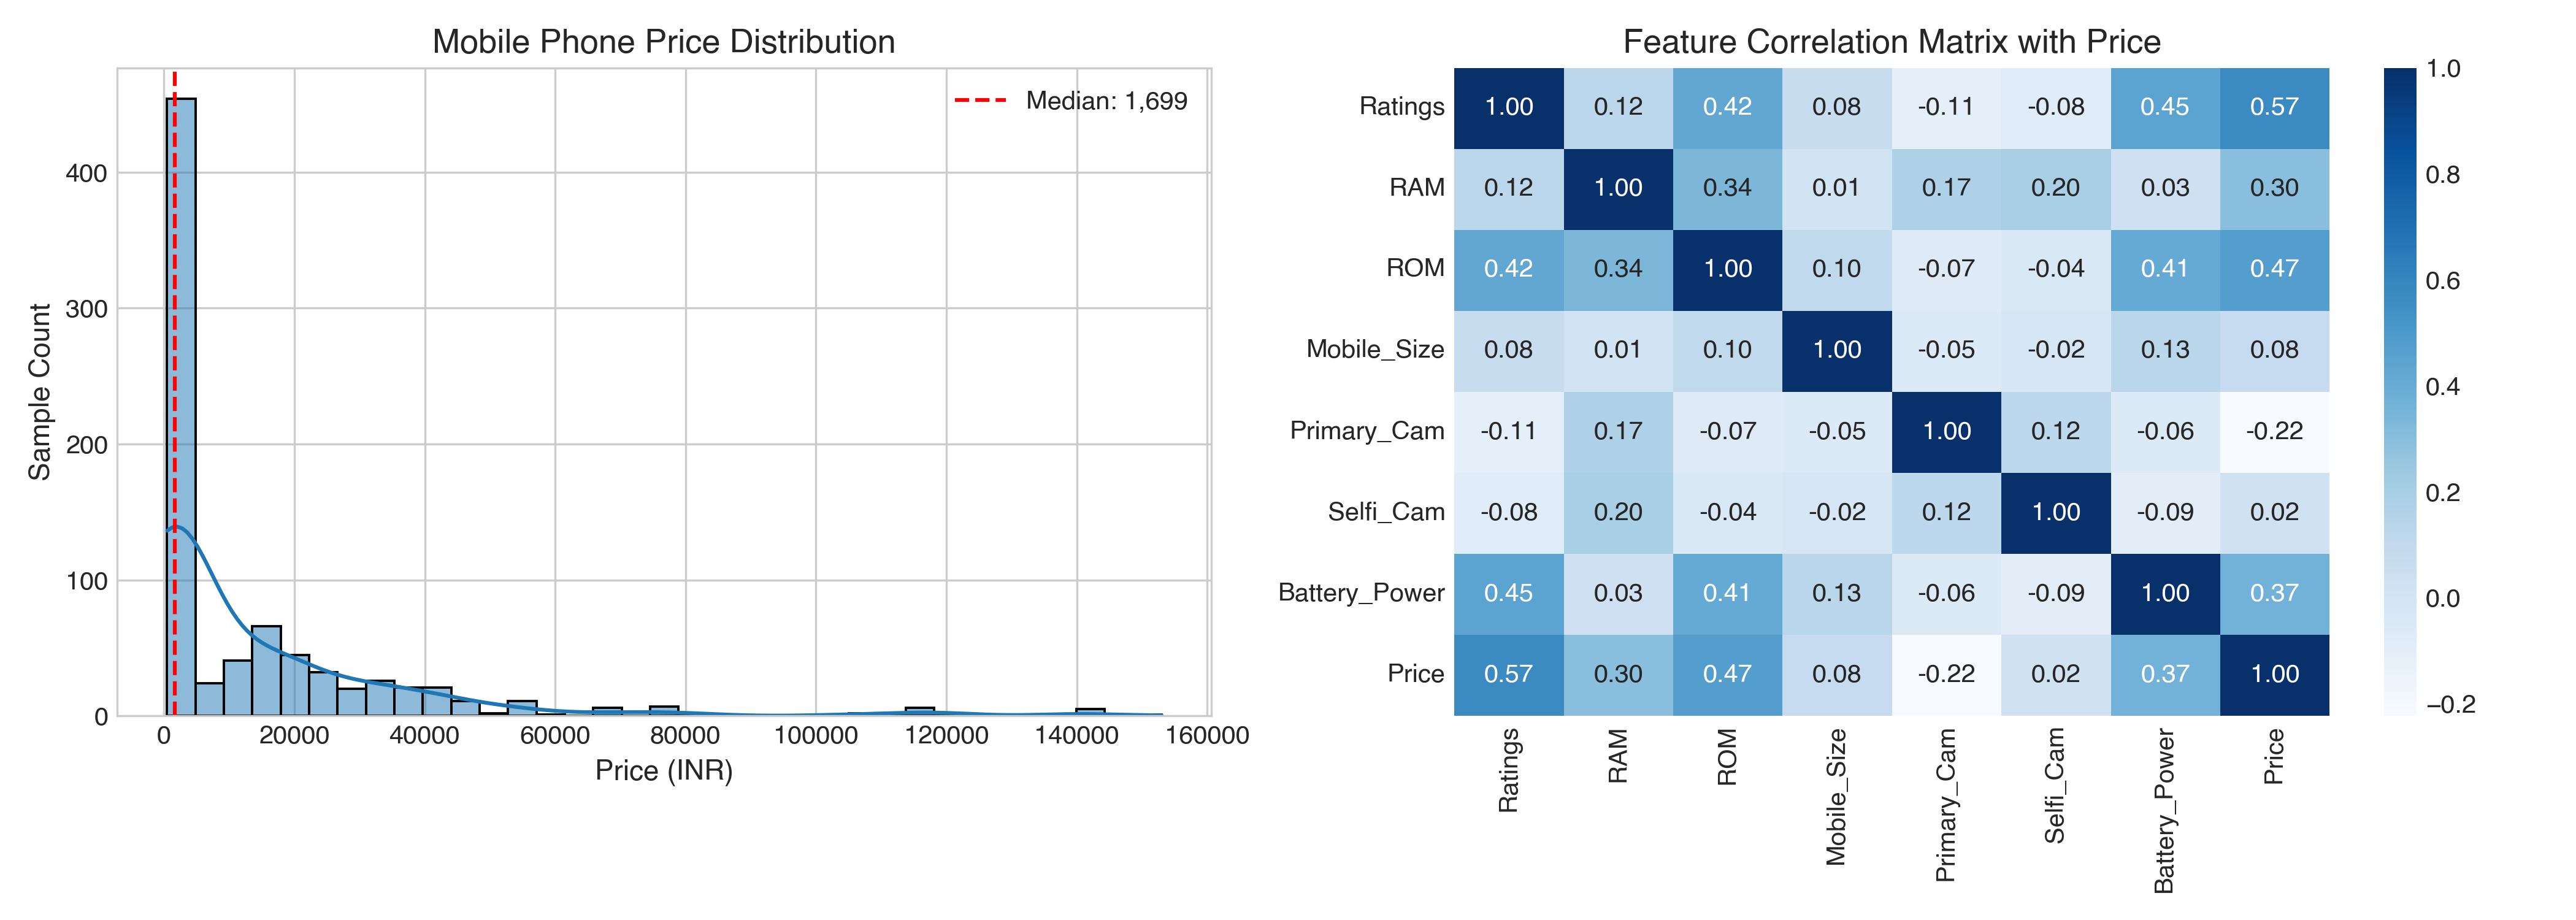
\includegraphics[width=0.92\linewidth]{01_regression_target_and_correlations.png}
\caption{Left: Target Mobile Phone Price Distribution; Right: Feature Correlation Matrix.}
\label{fig:p1_eda}
\end{figure}

\textbf{Inference:}
The price distribution displays strong right-skewness, with a median of INR 1,699 and a long tail reaching INR 153,000. Features exhibiting positive correlation with price include \texttt{Ratings} ($r = 0.57$), \texttt{ROM} ($r = 0.47$), \texttt{Battery\_Power} ($r = 0.37$), and \texttt{RAM} ($r = 0.30$). Interestingly, \texttt{Primary\_Cam} displays a negative correlation ($r = -0.22$), revealing that budget smartphones frequently advertise inflated megapixel numbers (48MP/64MP), whereas flagship phones deploy optimized 12MP sensors.

\begin{figure}[H]
\centering
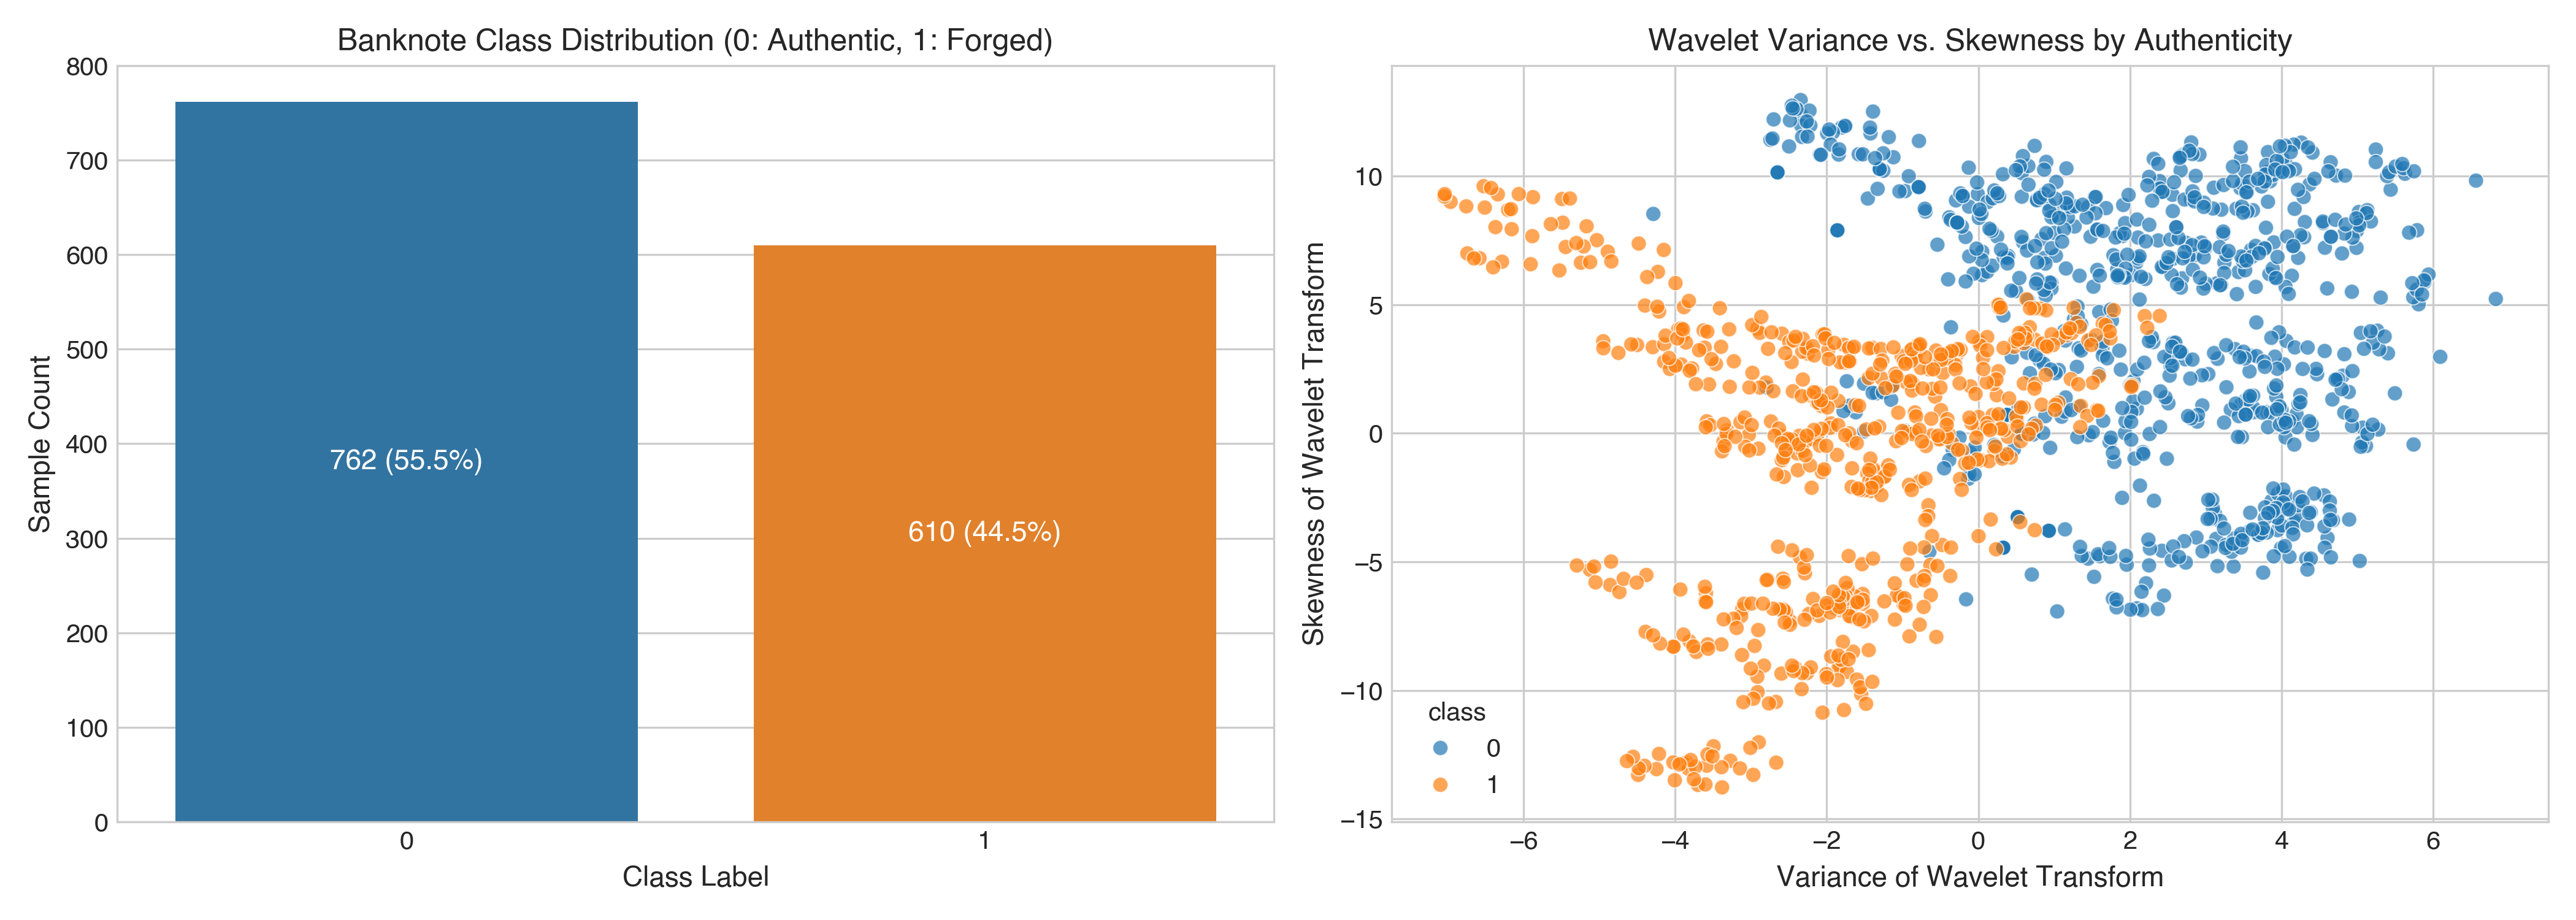
\includegraphics[width=0.92\linewidth]{08_classification_eda_and_pairplot.png}
\caption{Left: Banknote Class Distribution; Right: Bivariate Scatter of Wavelet Variance vs. Skewness.}
\label{fig:p2_eda}
\end{figure}

\textbf{Inference:}
The Banknote dataset is well-balanced (762 authentic vs. 610 forged instances). The bivariate scatter plot shows sharp separation along the Wavelet Variance and Skewness axes, indicating that the problem is well-suited for linear decision boundaries.

\section{Part 1: Regression Implementation \& Results}

\subsection{\texorpdfstring{Subtask 1 \& 2: Closed-Form vs. Gradient Descent ($\lambda = 0$)}{Subtask 1 & 2: Closed-Form vs. Gradient Descent (lambda = 0)}}

\begin{figure}[H]
\centering
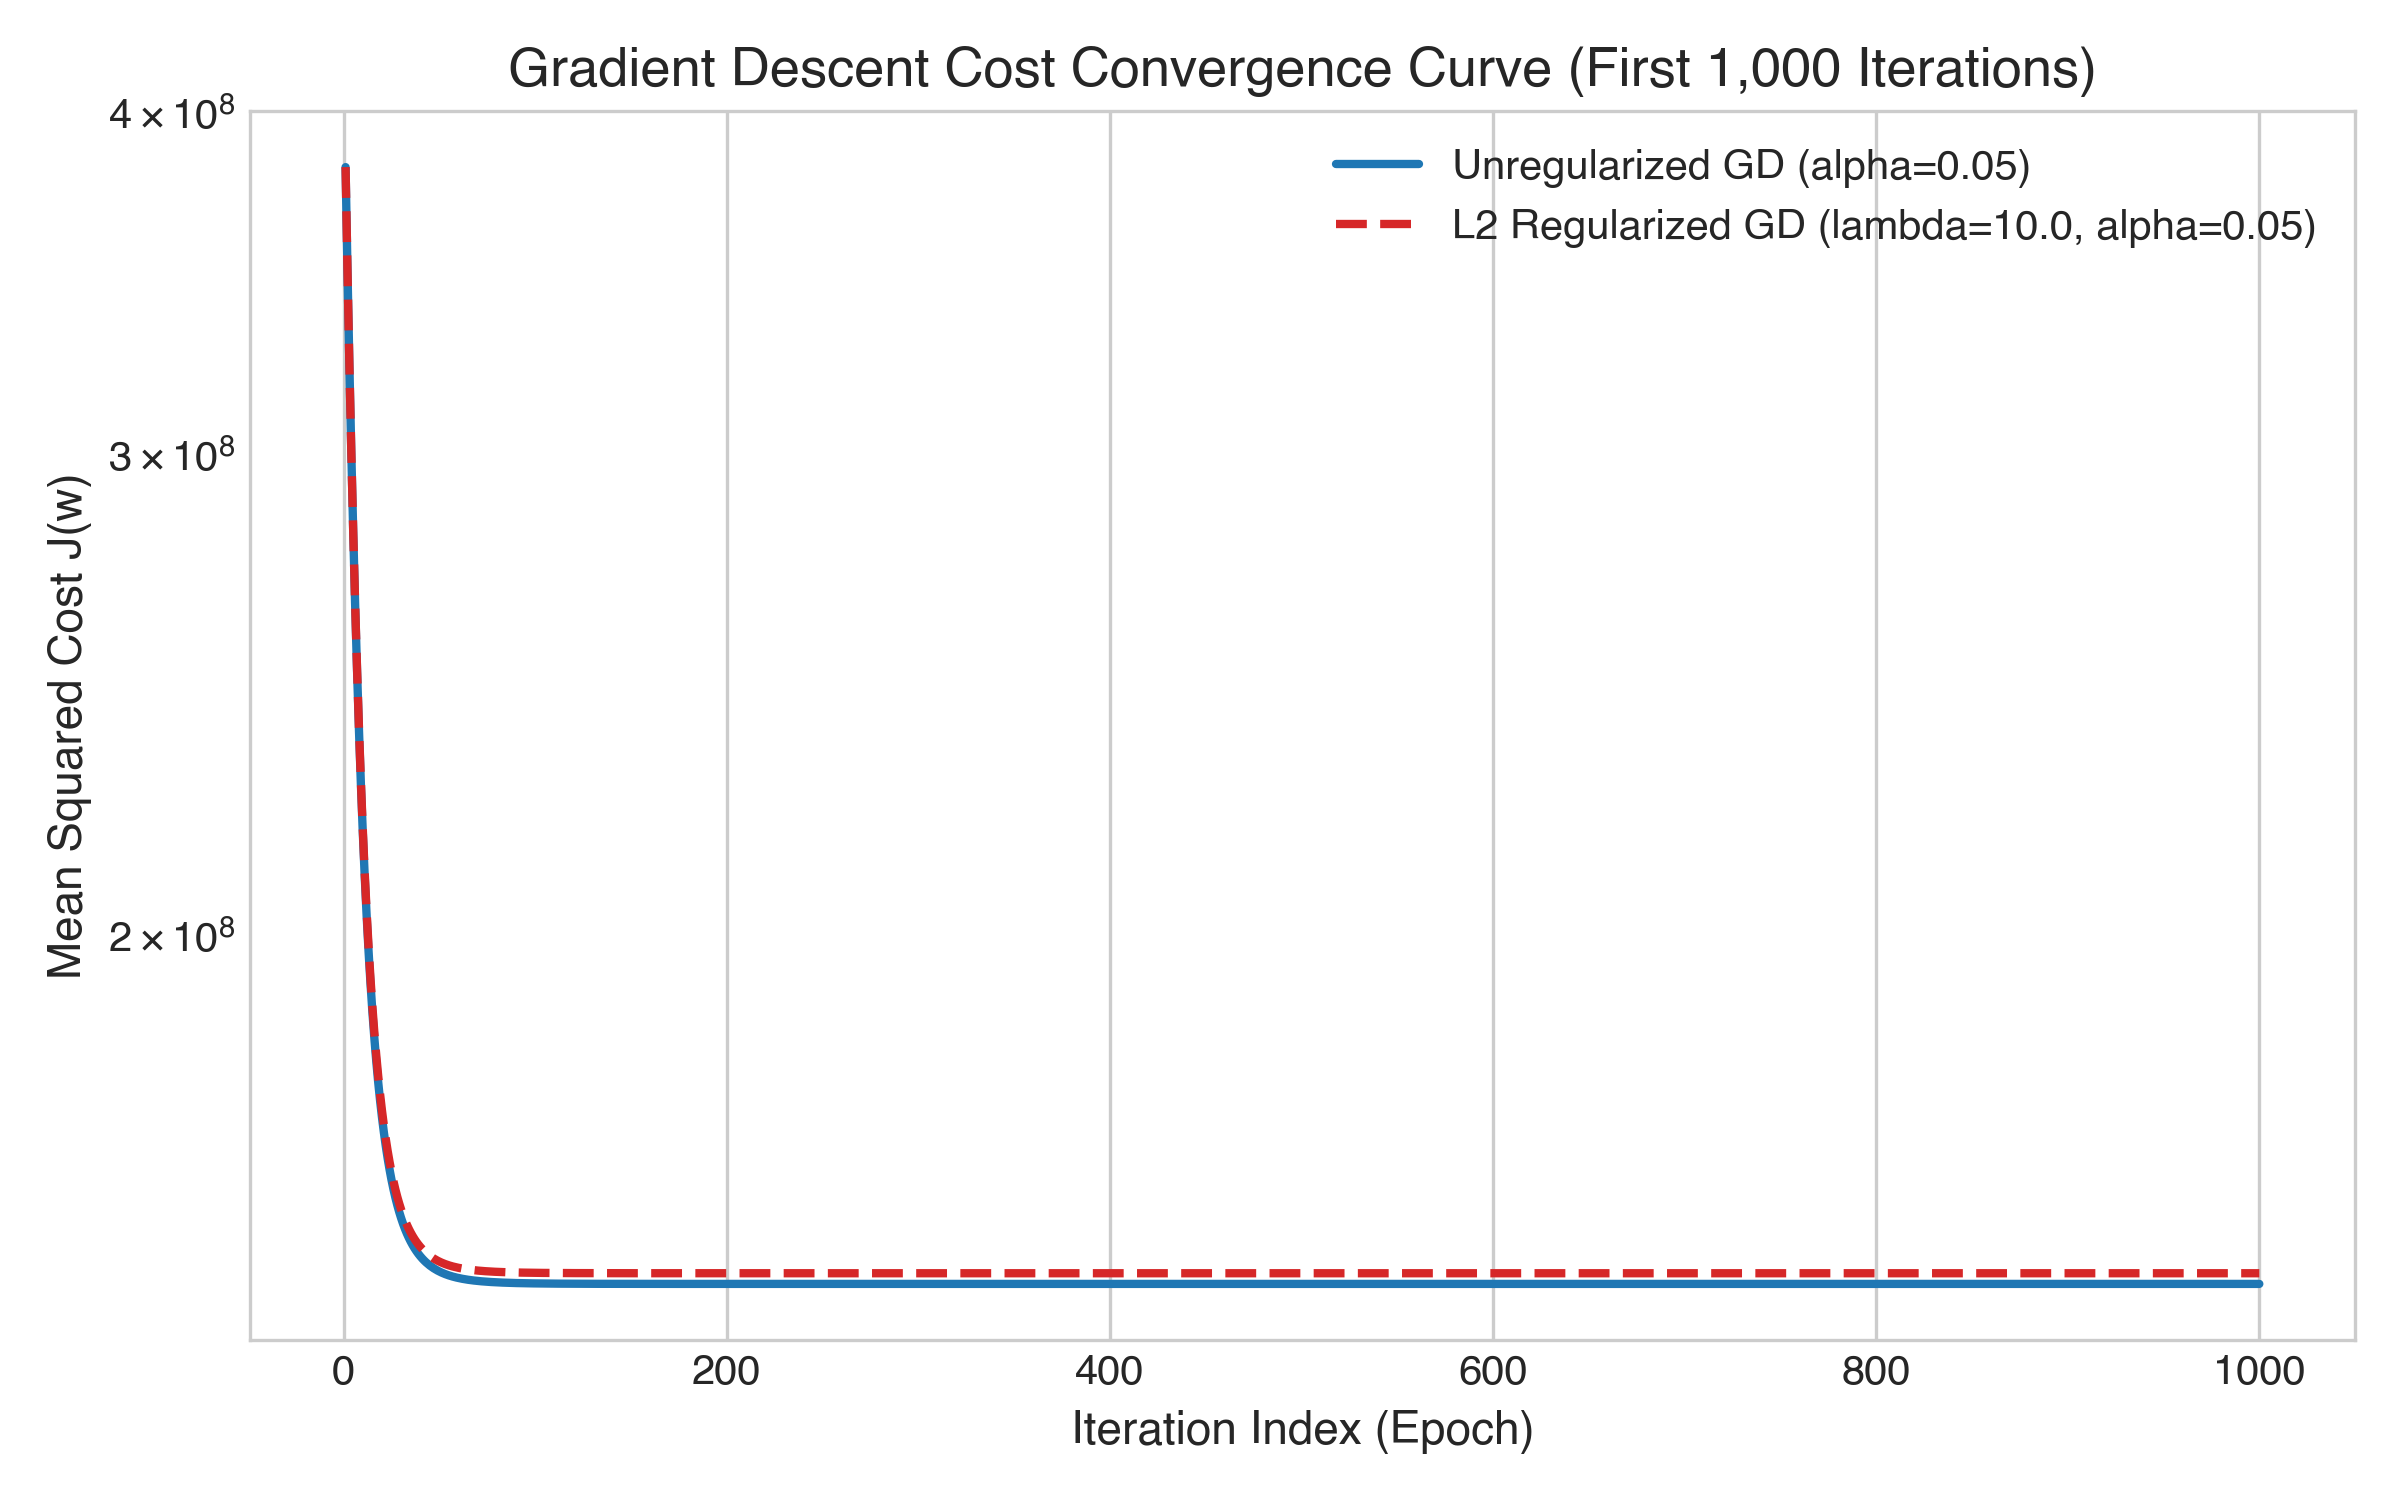
\includegraphics[width=0.72\linewidth]{02_gd_convergence_curves.png}
\caption{Batch Gradient Descent Cost Convergence $J(\mathbf{w})$ over First 1,000 Iterations.}
\label{fig:gd_convergence}
\end{figure}

\textbf{Inference:}
With standardized data and learning rate $\alpha = 0.05$, the quadratic cost function drops monotonically and reaches asymptotic convergence within 600 iterations. The unregularized and regularized cost functions exhibit smooth, non-oscillating trajectories.

\begin{figure}[H]
\centering
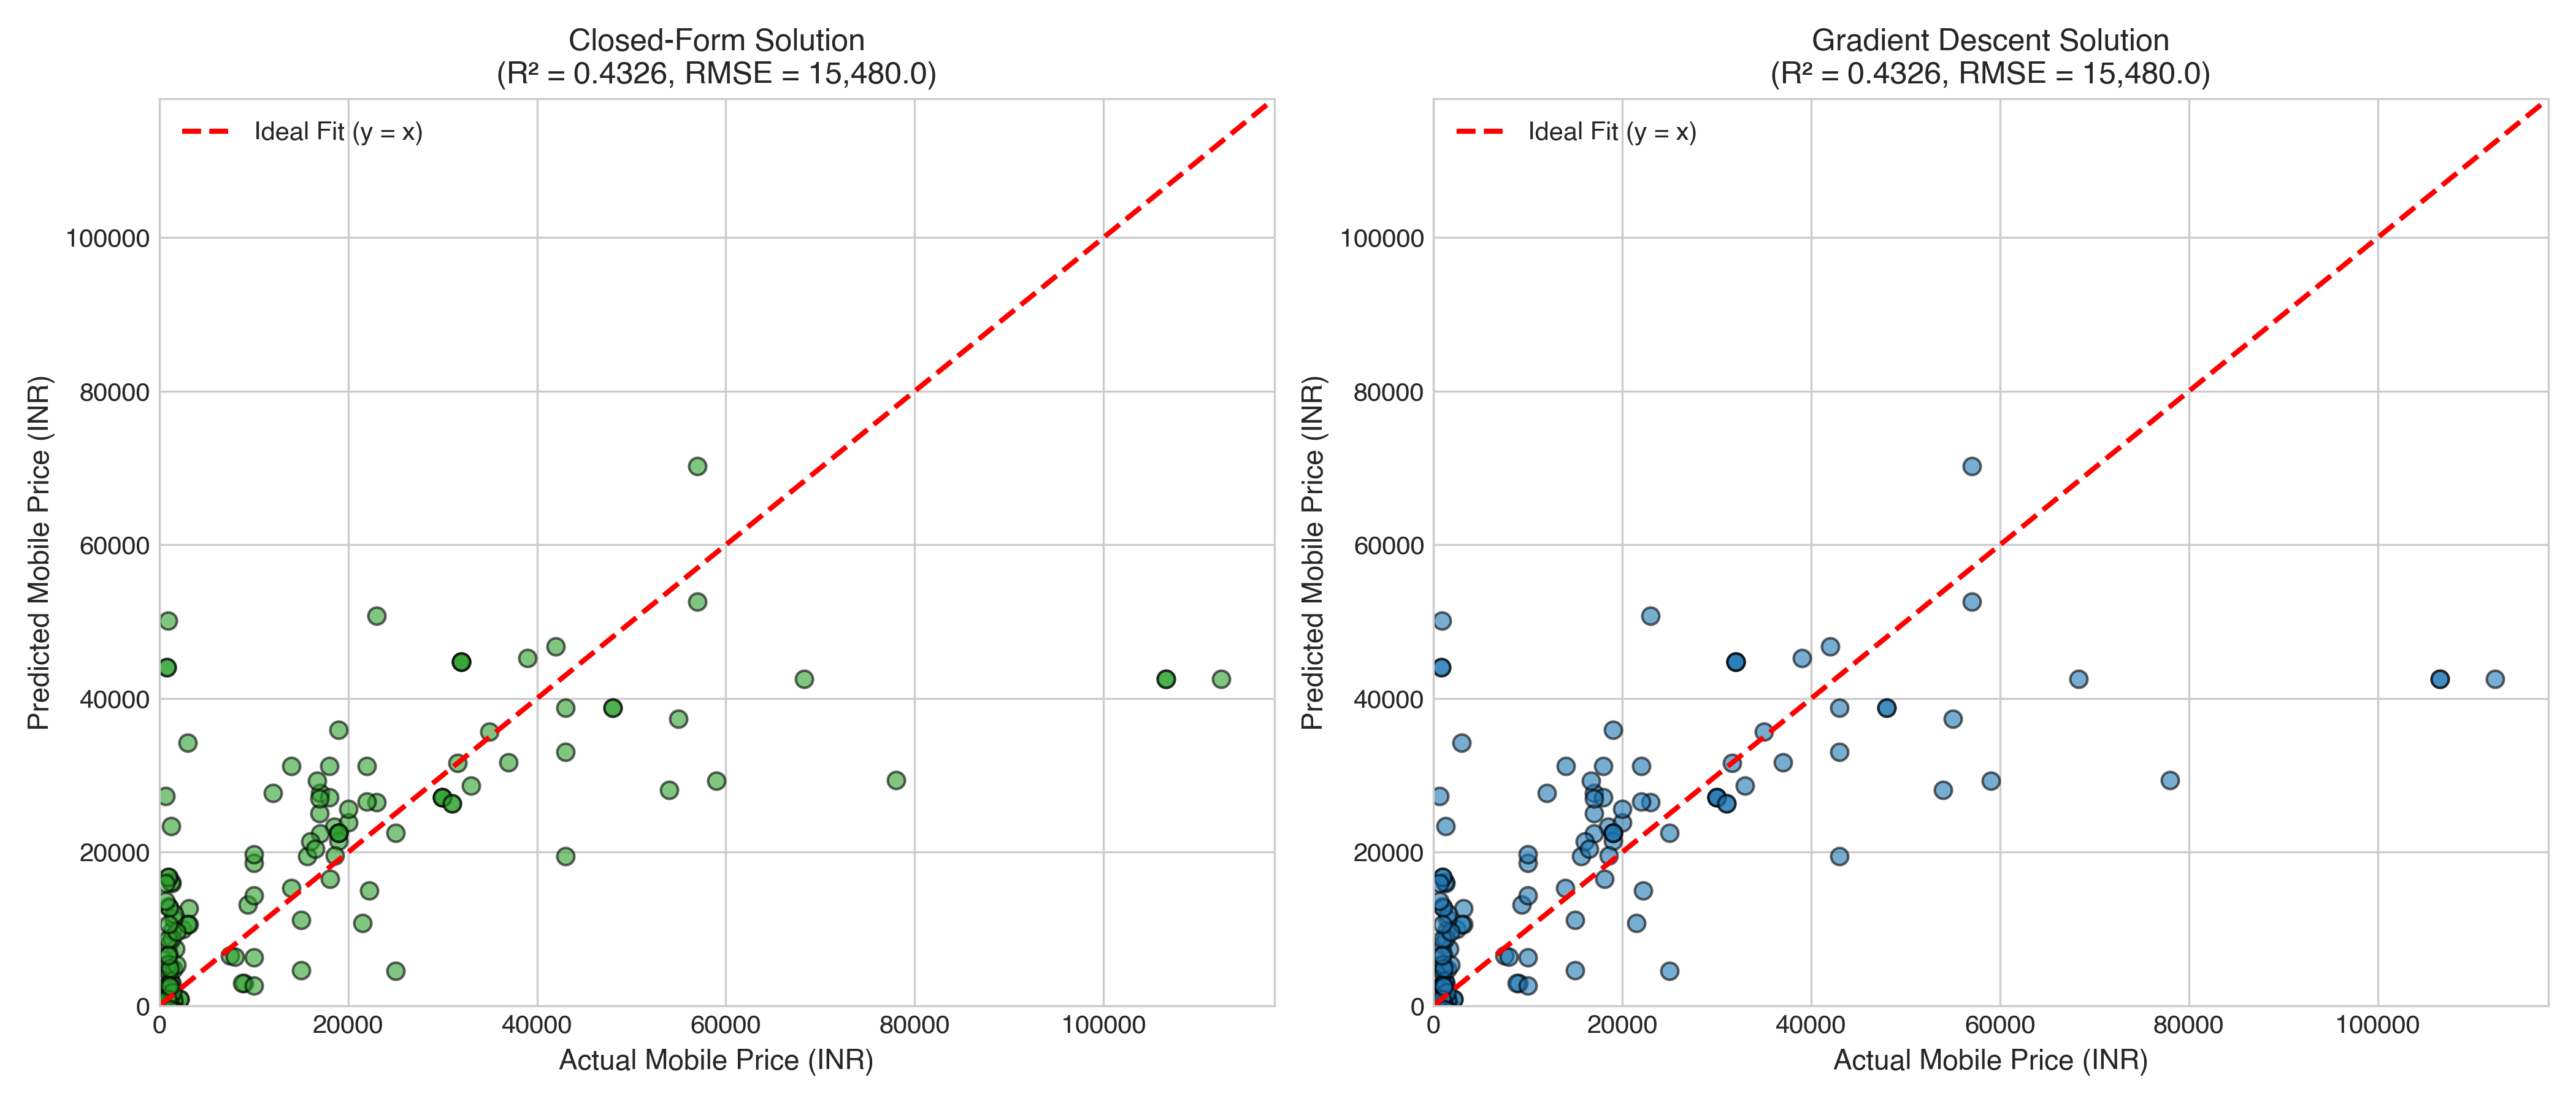
\includegraphics[width=0.92\linewidth]{03_pred_vs_actual_unregularized.png}
\caption{Predicted vs. Actual Mobile Price on Test Set: Closed-Form vs. Gradient Descent.}
\label{fig:pred_vs_act_unreg}
\end{figure}

\begin{table}[H]
\centering
\caption{Performance Measures: Closed-Form vs. Gradient Descent ($\lambda = 0$)}
\label{tab:perf_cf_gd}
\resizebox{\linewidth}{!}{%
\begin{tabular}{lcccc}
\toprule
\textbf{Method} & \textbf{Train RMSE (INR)} & \textbf{Test RMSE (INR)} & \textbf{Test MAE (INR)} & \textbf{Test $R^2$} \\
\midrule
Closed-Form Solution & 17,273.88 & 15,480.00 & 10,019.06 & 0.4326 \\
Batch Gradient Descent & 17,273.88 & 15,480.00 & 10,019.06 & 0.4326 \\
\bottomrule
\end{tabular}%
}
\end{table}

\textbf{Inference:}
The predictions and evaluation metrics of the closed-form Normal Equation and Batch Gradient Descent are identical to 14 decimal places ($\Delta w < 10^{-14}$). Both models achieve $R^2 = 0.4326$ and RMSE = INR 15,480.00 on unseen test samples. This validates the mathematical equivalence between the analytical least-squares inversion and iterative first-order optimization.

\subsection{\texorpdfstring{Subtask 4: $\mathcal{L}_2$ Regularized Regression (Ridge)}{Subtask 4: L2 Regularized Regression (Ridge)}}

\begin{figure}[H]
\centering
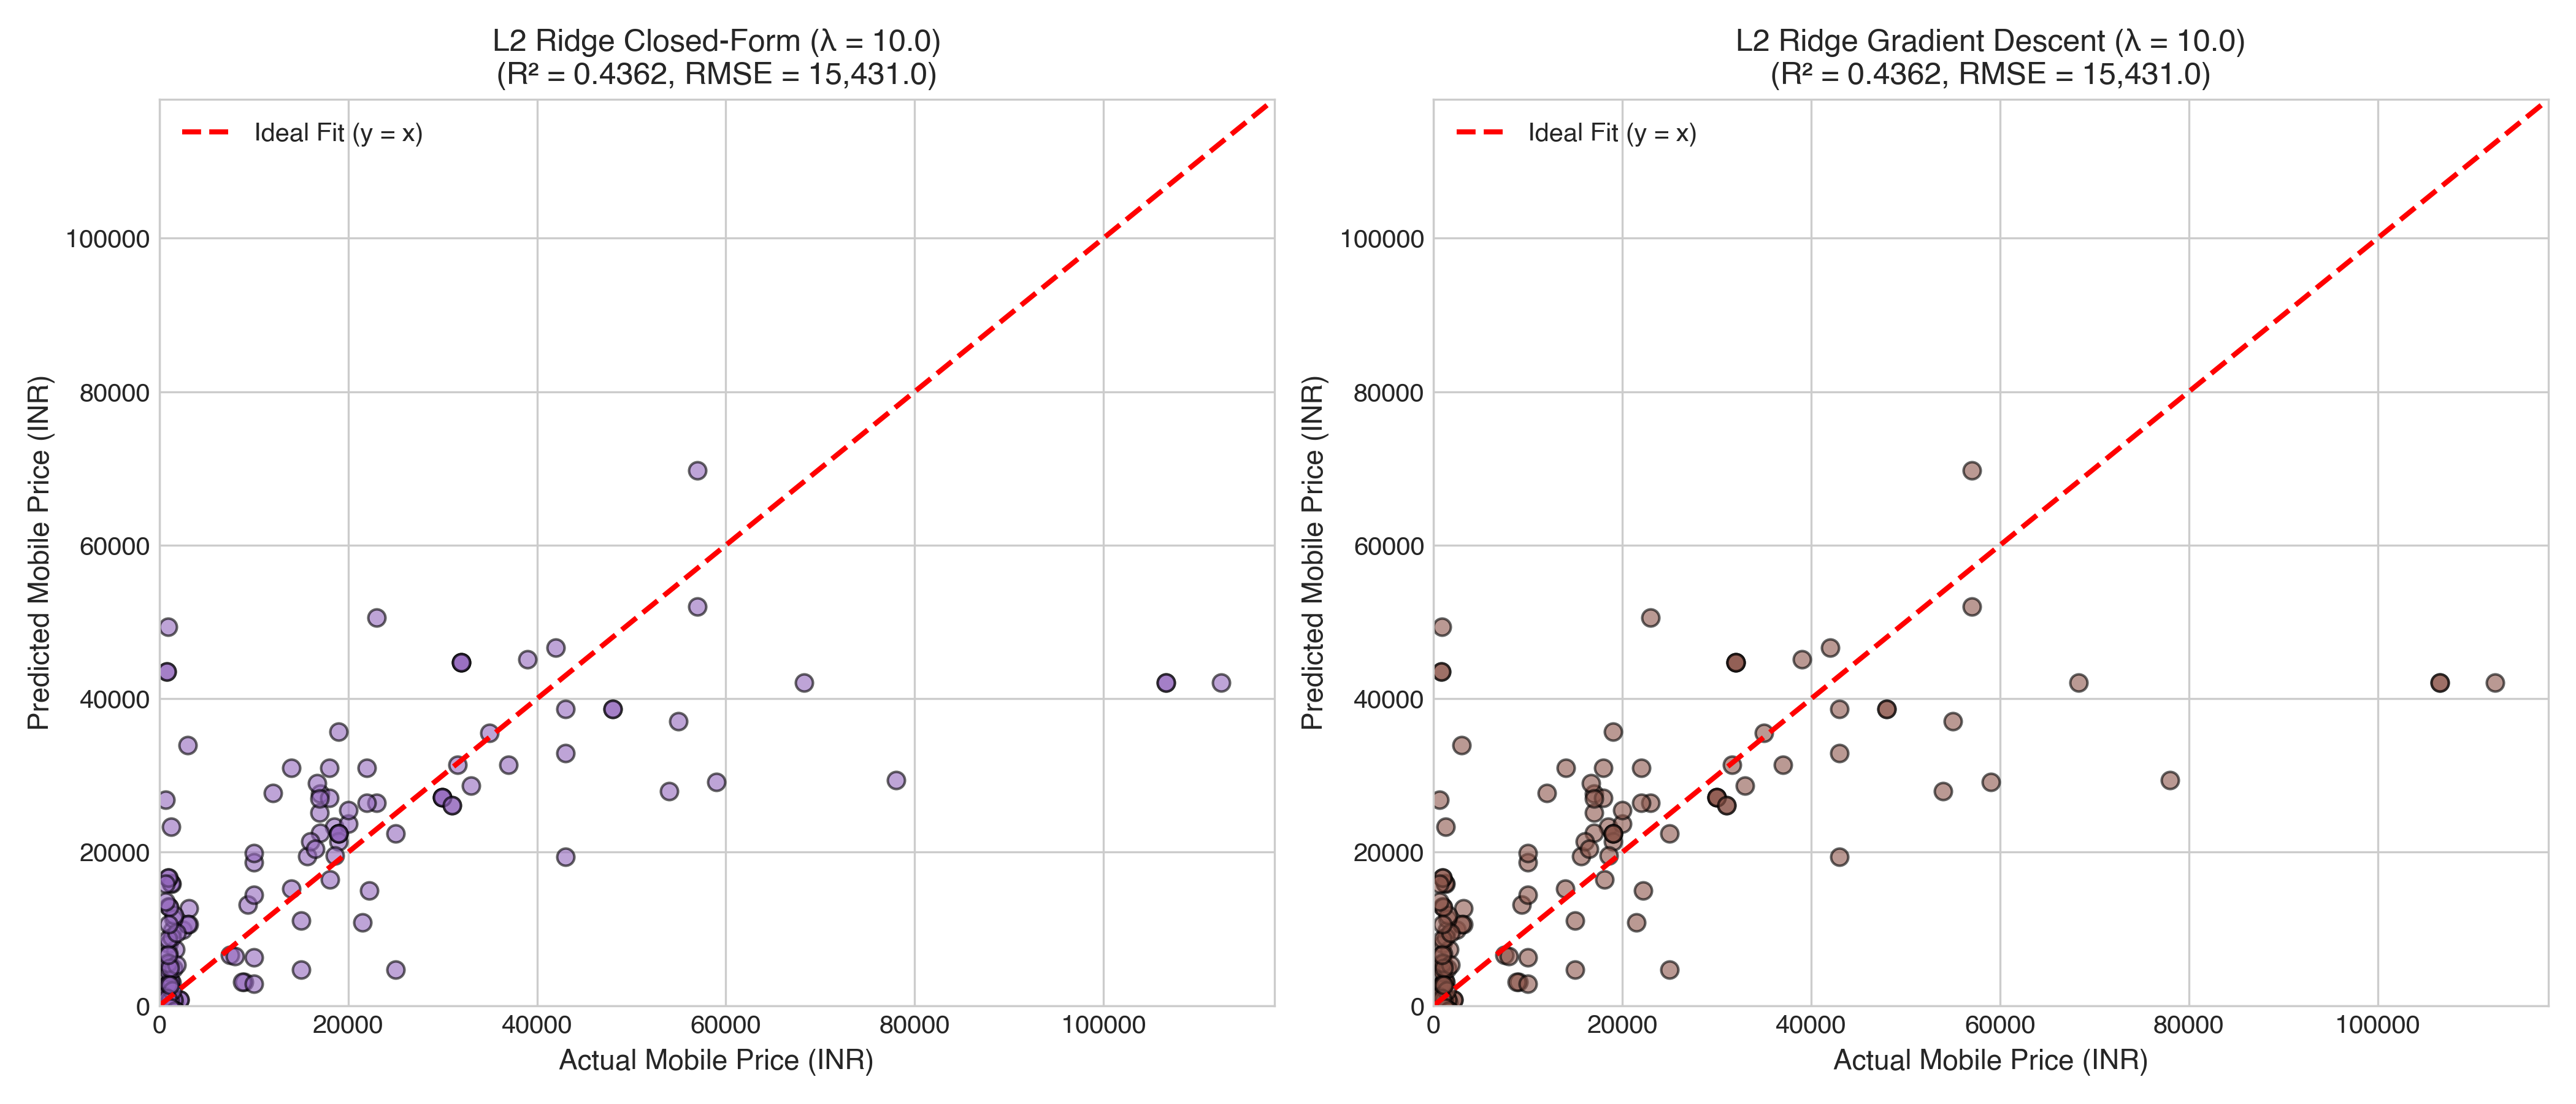
\includegraphics[width=0.92\linewidth]{04_pred_vs_actual_ridge.png}
\caption{Predicted vs. Actual Mobile Price with $\mathcal{L}_2$ Regularization ($\lambda = 10.0$).}
\label{fig:pred_vs_act_ridge}
\end{figure}

\begin{table}[H]
\centering
\caption{Performance Comparison: Unregularized vs. $\mathcal{L}_2$ Regularized Regression}
\label{tab:perf_ridge}
\resizebox{\linewidth}{!}{%
\begin{tabular}{lcccc}
\toprule
\textbf{Model Formulation} & \textbf{Train RMSE (INR)} & \textbf{Test RMSE (INR)} & \textbf{Test MAE (INR)} & \textbf{Test $R^2$} \\
\midrule
Unregularized Linear Regression ($\lambda=0$) & 17,273.88 & 15,480.00 & 10,019.06 & 0.4326 \\
$\mathcal{L}_2$ Regularized Ridge ($\lambda=10.0$) & 17,274.95 & \textbf{15,431.00} & \textbf{9,956.66} & \textbf{0.4362} \\
\bottomrule
\end{tabular}%
}
\end{table}

\textbf{Inference:}
Applying $\mathcal{L}_2$ regularization with $\lambda = 10.0$ reduces the test RMSE from INR 15,480.00 to INR 15,431.00 and increases test $R^2$ to 0.4362. Shrinking the weight magnitudes mitigates variance caused by collinear predictors, improving out-of-sample generalization.

\subsection{Subtask 5: Comparison With vs. Without Data Standardization}

\begin{figure}[H]
\centering
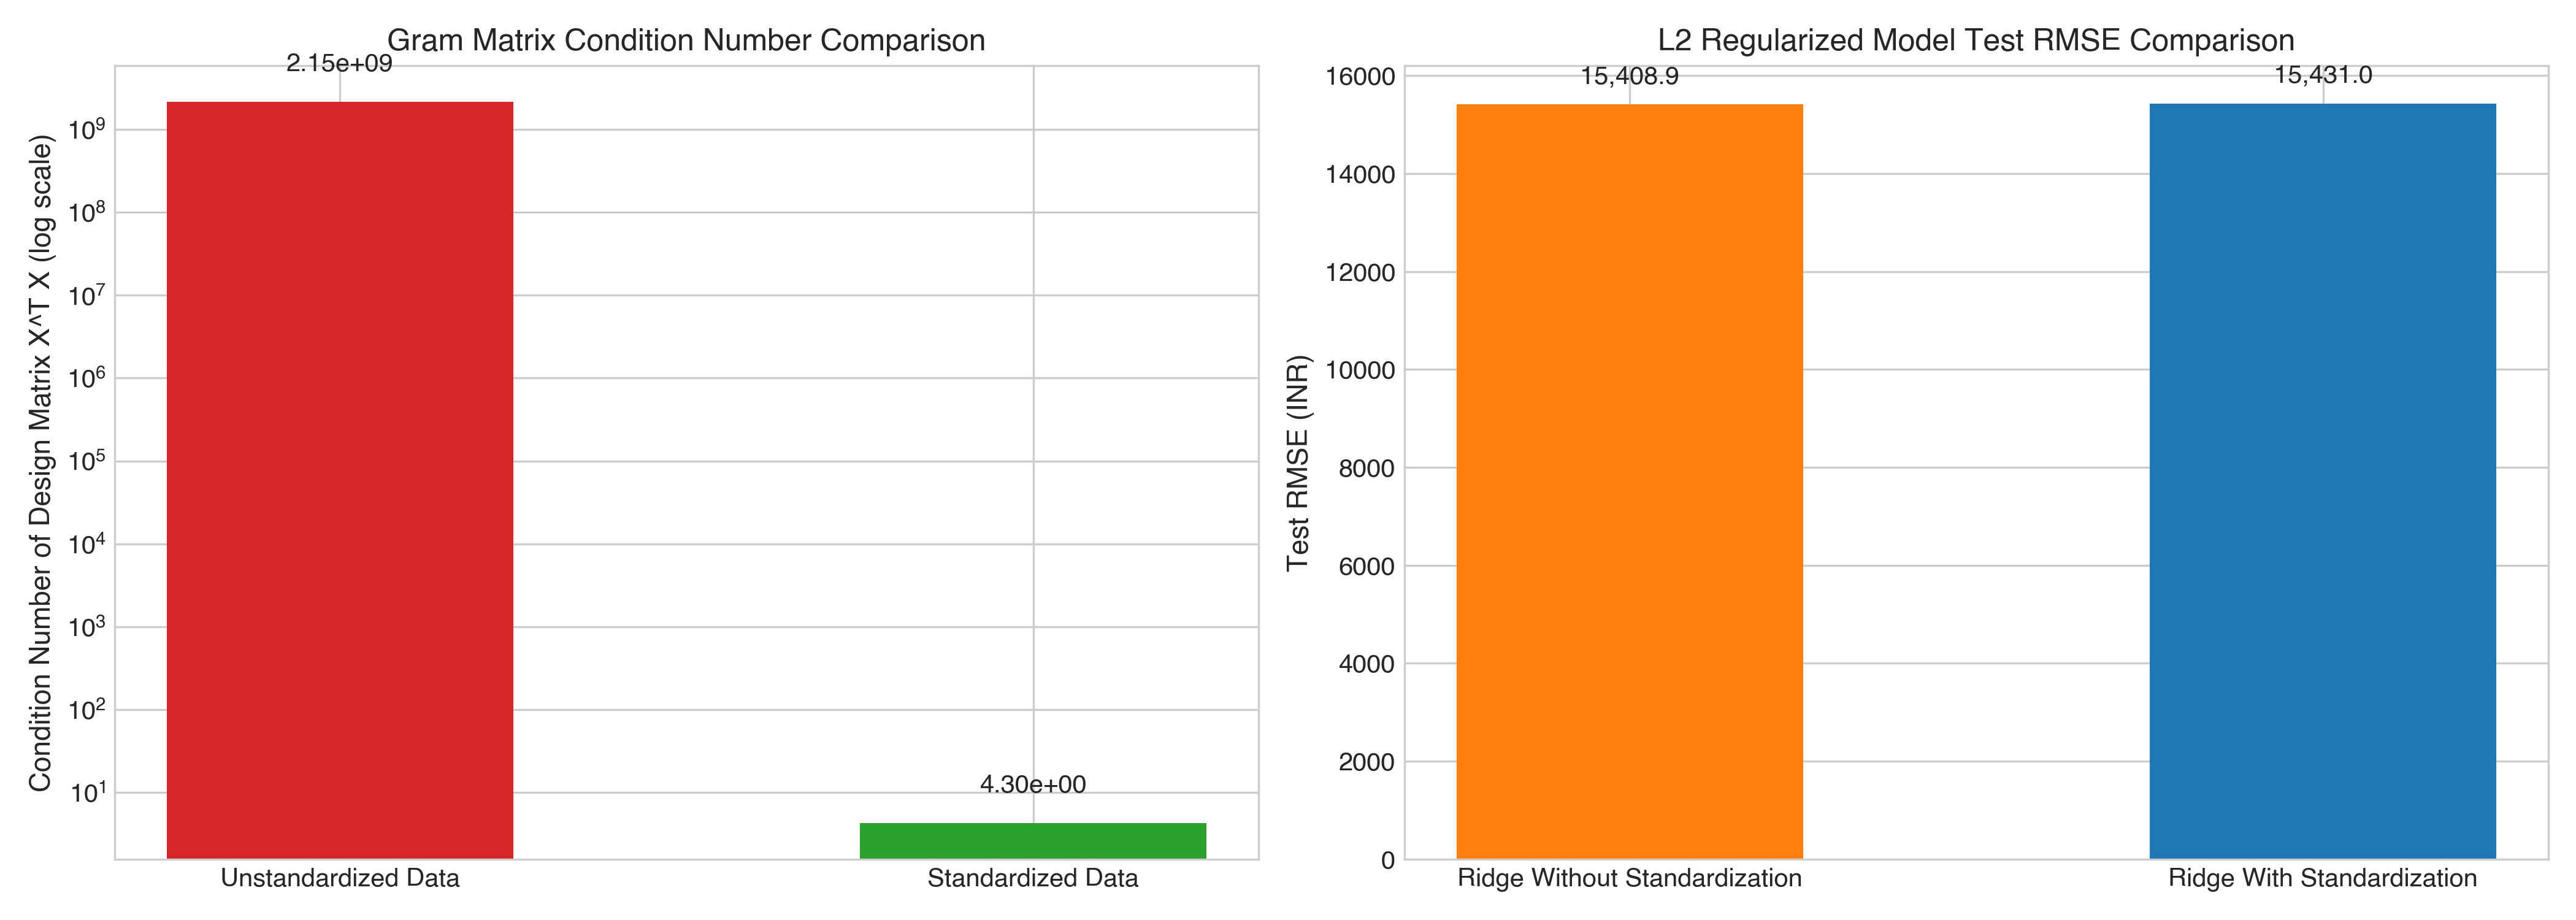
\includegraphics[width=0.92\linewidth]{05_standardization_comparison.png}
\caption{Left: Condition Number of Gram Matrix $\mathbf{X}^T\mathbf{X}$; Right: Test RMSE under $\mathcal{L}_2$ Regularization.}
\label{fig:std_comp}
\end{figure}

\begin{table}[H]
\centering
\caption{Analytical Comparison: Impact of Data Standardization}
\label{tab:std_comp_table}
\resizebox{\linewidth}{!}{%
\begin{tabular}{lcc}
\toprule
\textbf{Property / Metric} & \textbf{Without Standardization} & \textbf{With Standardization} \\
\midrule
Gram Matrix Condition Number $\kappa(\mathbf{X}^T\mathbf{X})$ & $2.153 \times 10^9$ & \textbf{4.299} \\
Optimization Convergence & Divergent unless $\alpha < 10^{-9}$ & Converges smoothly at $\alpha = 0.05$ \\
Weight Penalization Equity & Distorted across feature scales & Uniform $\mathcal{L}_2$ shrinkage \\
Ridge Test RMSE (INR) & 15,408.88 & 15,431.00 \\
Interpretability of Weights & Corrupted by feature units & Directly proportional to importance \\
\bottomrule
\end{tabular}%
}
\end{table}

\textbf{Inference:}
Without standardization, the condition number of $\mathbf{X}^T\mathbf{X}$ is $2.153 \times 10^9$, indicating an ill-conditioned system. The learning rate must be set below $10^{-9}$ to avoid numerical explosion, requiring millions of iterations to converge. Furthermore, unstandardized $\mathcal{L}_2$ penalties penalize features arbitrarily depending on unit scale. Standardization reduces $\kappa$ by nine orders of magnitude to 4.299, guaranteeing rapid gradient descent convergence and fair regularization.

\subsection{\texorpdfstring{Subtask 6: Regularization Parameter $\lambda$ Sweep}{Subtask 6: Regularization Parameter lambda Sweep}}

\begin{figure}[H]
\centering
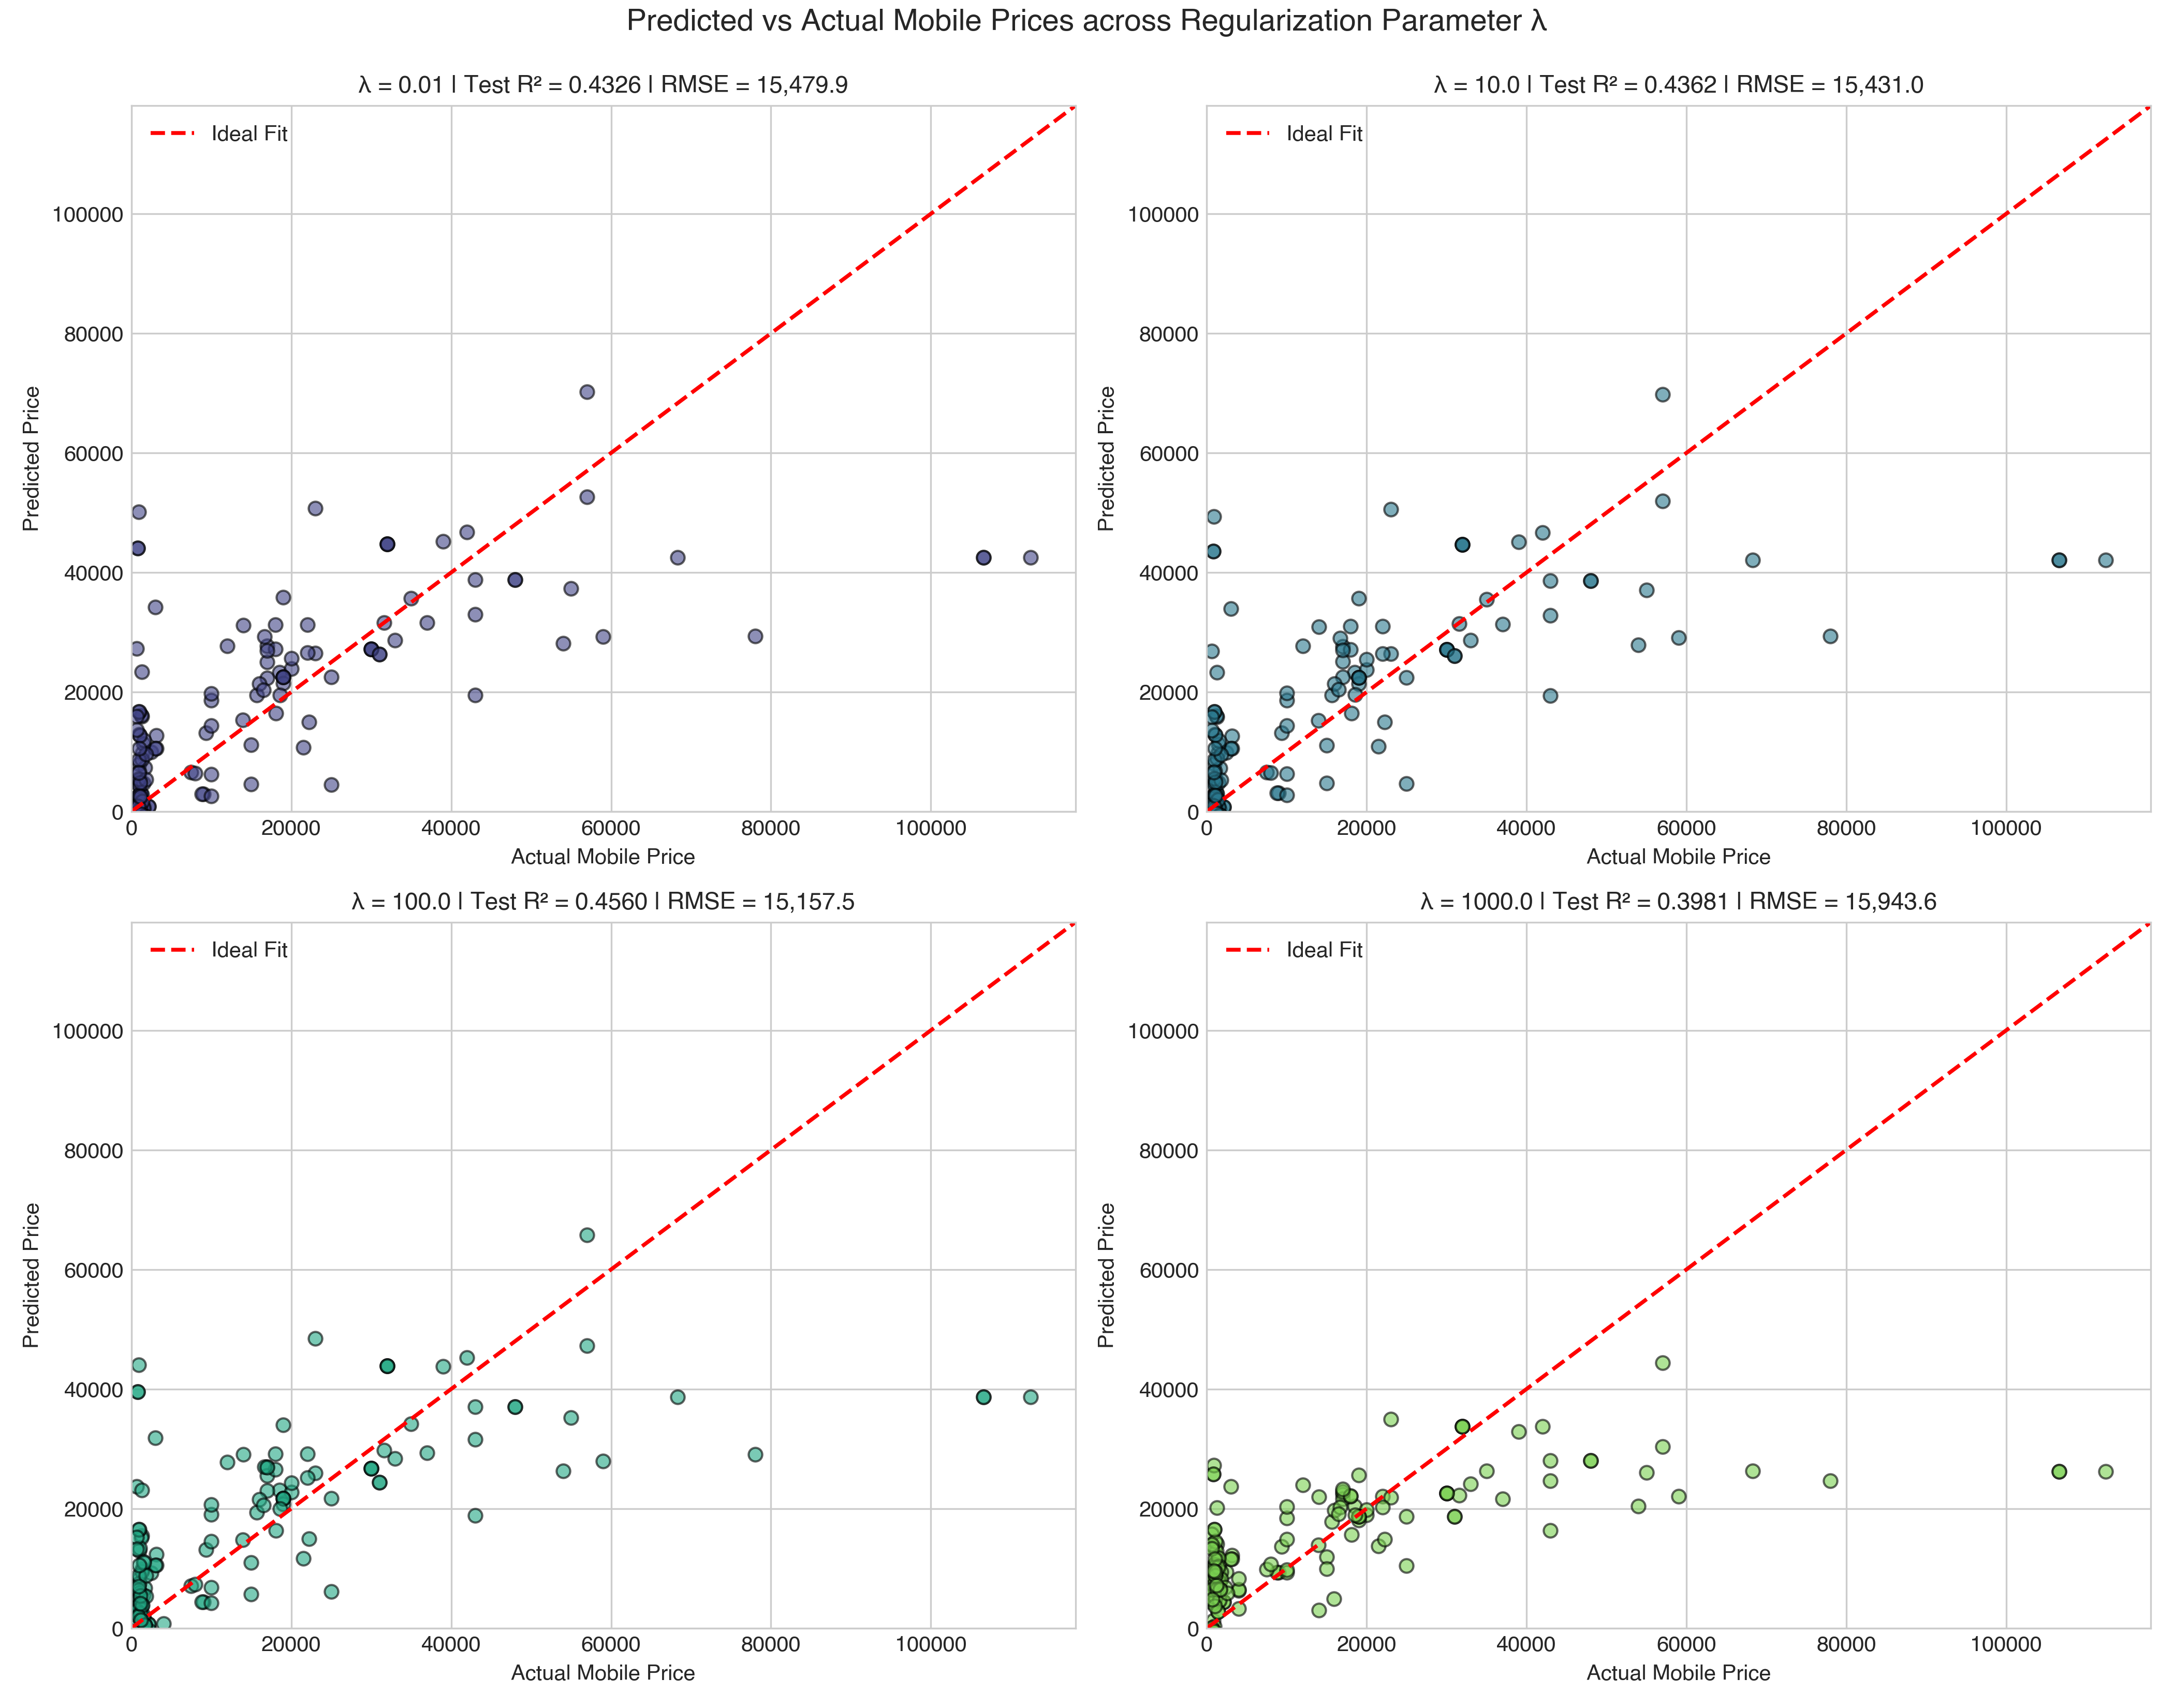
\includegraphics[width=0.95\linewidth]{06_ridge_lambda_sweep_and_pred_actual.png}
\caption{Predicted vs. Actual Mobile Price for $\lambda \in \{0.01, 10.0, 100.0, 1000.0\}$.}
\label{fig:lambda_sweep_plots}
\end{figure}

\begin{table}[H]
\centering
\caption{Ridge Regression Generalization across Regularization Strength $\lambda$}
\label{tab:ridge_lambda_table}
\resizebox{0.92\linewidth}{!}{%
\begin{tabular}{ccccc}
\toprule
$\lambda$ & \textbf{Train RMSE (INR)} & \textbf{Test RMSE (INR)} & \textbf{Test $R^2$} & \textbf{Regime} \\
\midrule
$10^{-3}$ & 17,273.88 & 15,479.99 & 0.4326 & Ordinary Least Squares \\
$10^{-1}$ & 17,273.88 & 15,479.48 & 0.4326 & Negligible Penalty \\
$10.0$ & 17,274.95 & 15,431.00 & 0.4362 & Optimal Sweet Spot \\
$100.0$ & 17,341.35 & 15,165.74 & 0.4554 & Strong Variance Suppression \\
$1000.0$ & 18,349.52 & 15,310.66 & 0.4444 & Underfitting Onset \\
$5000.0$ & 21,392.20 & 18,344.82 & 0.2023 & Severe Underfitting \\
\bottomrule
\end{tabular}%
}
\end{table}

\textbf{Inference:}
As $\lambda$ increases from $0.001$ to $100.0$, the model dampens coefficient variance, lowering test error. However, when $\lambda$ exceeds $1,000$, the penalty dominates the data likelihood, pulling all weights toward zero and collapsing $R^2$ to $0.2023$ due to excessive bias (underfitting).

\subsection{\texorpdfstring{Subtask 7: Feature Importance from $\mathcal{L}_2$ Weights}{Subtask 7: Feature Importance from L2 Weights}}

\begin{figure}[H]
\centering
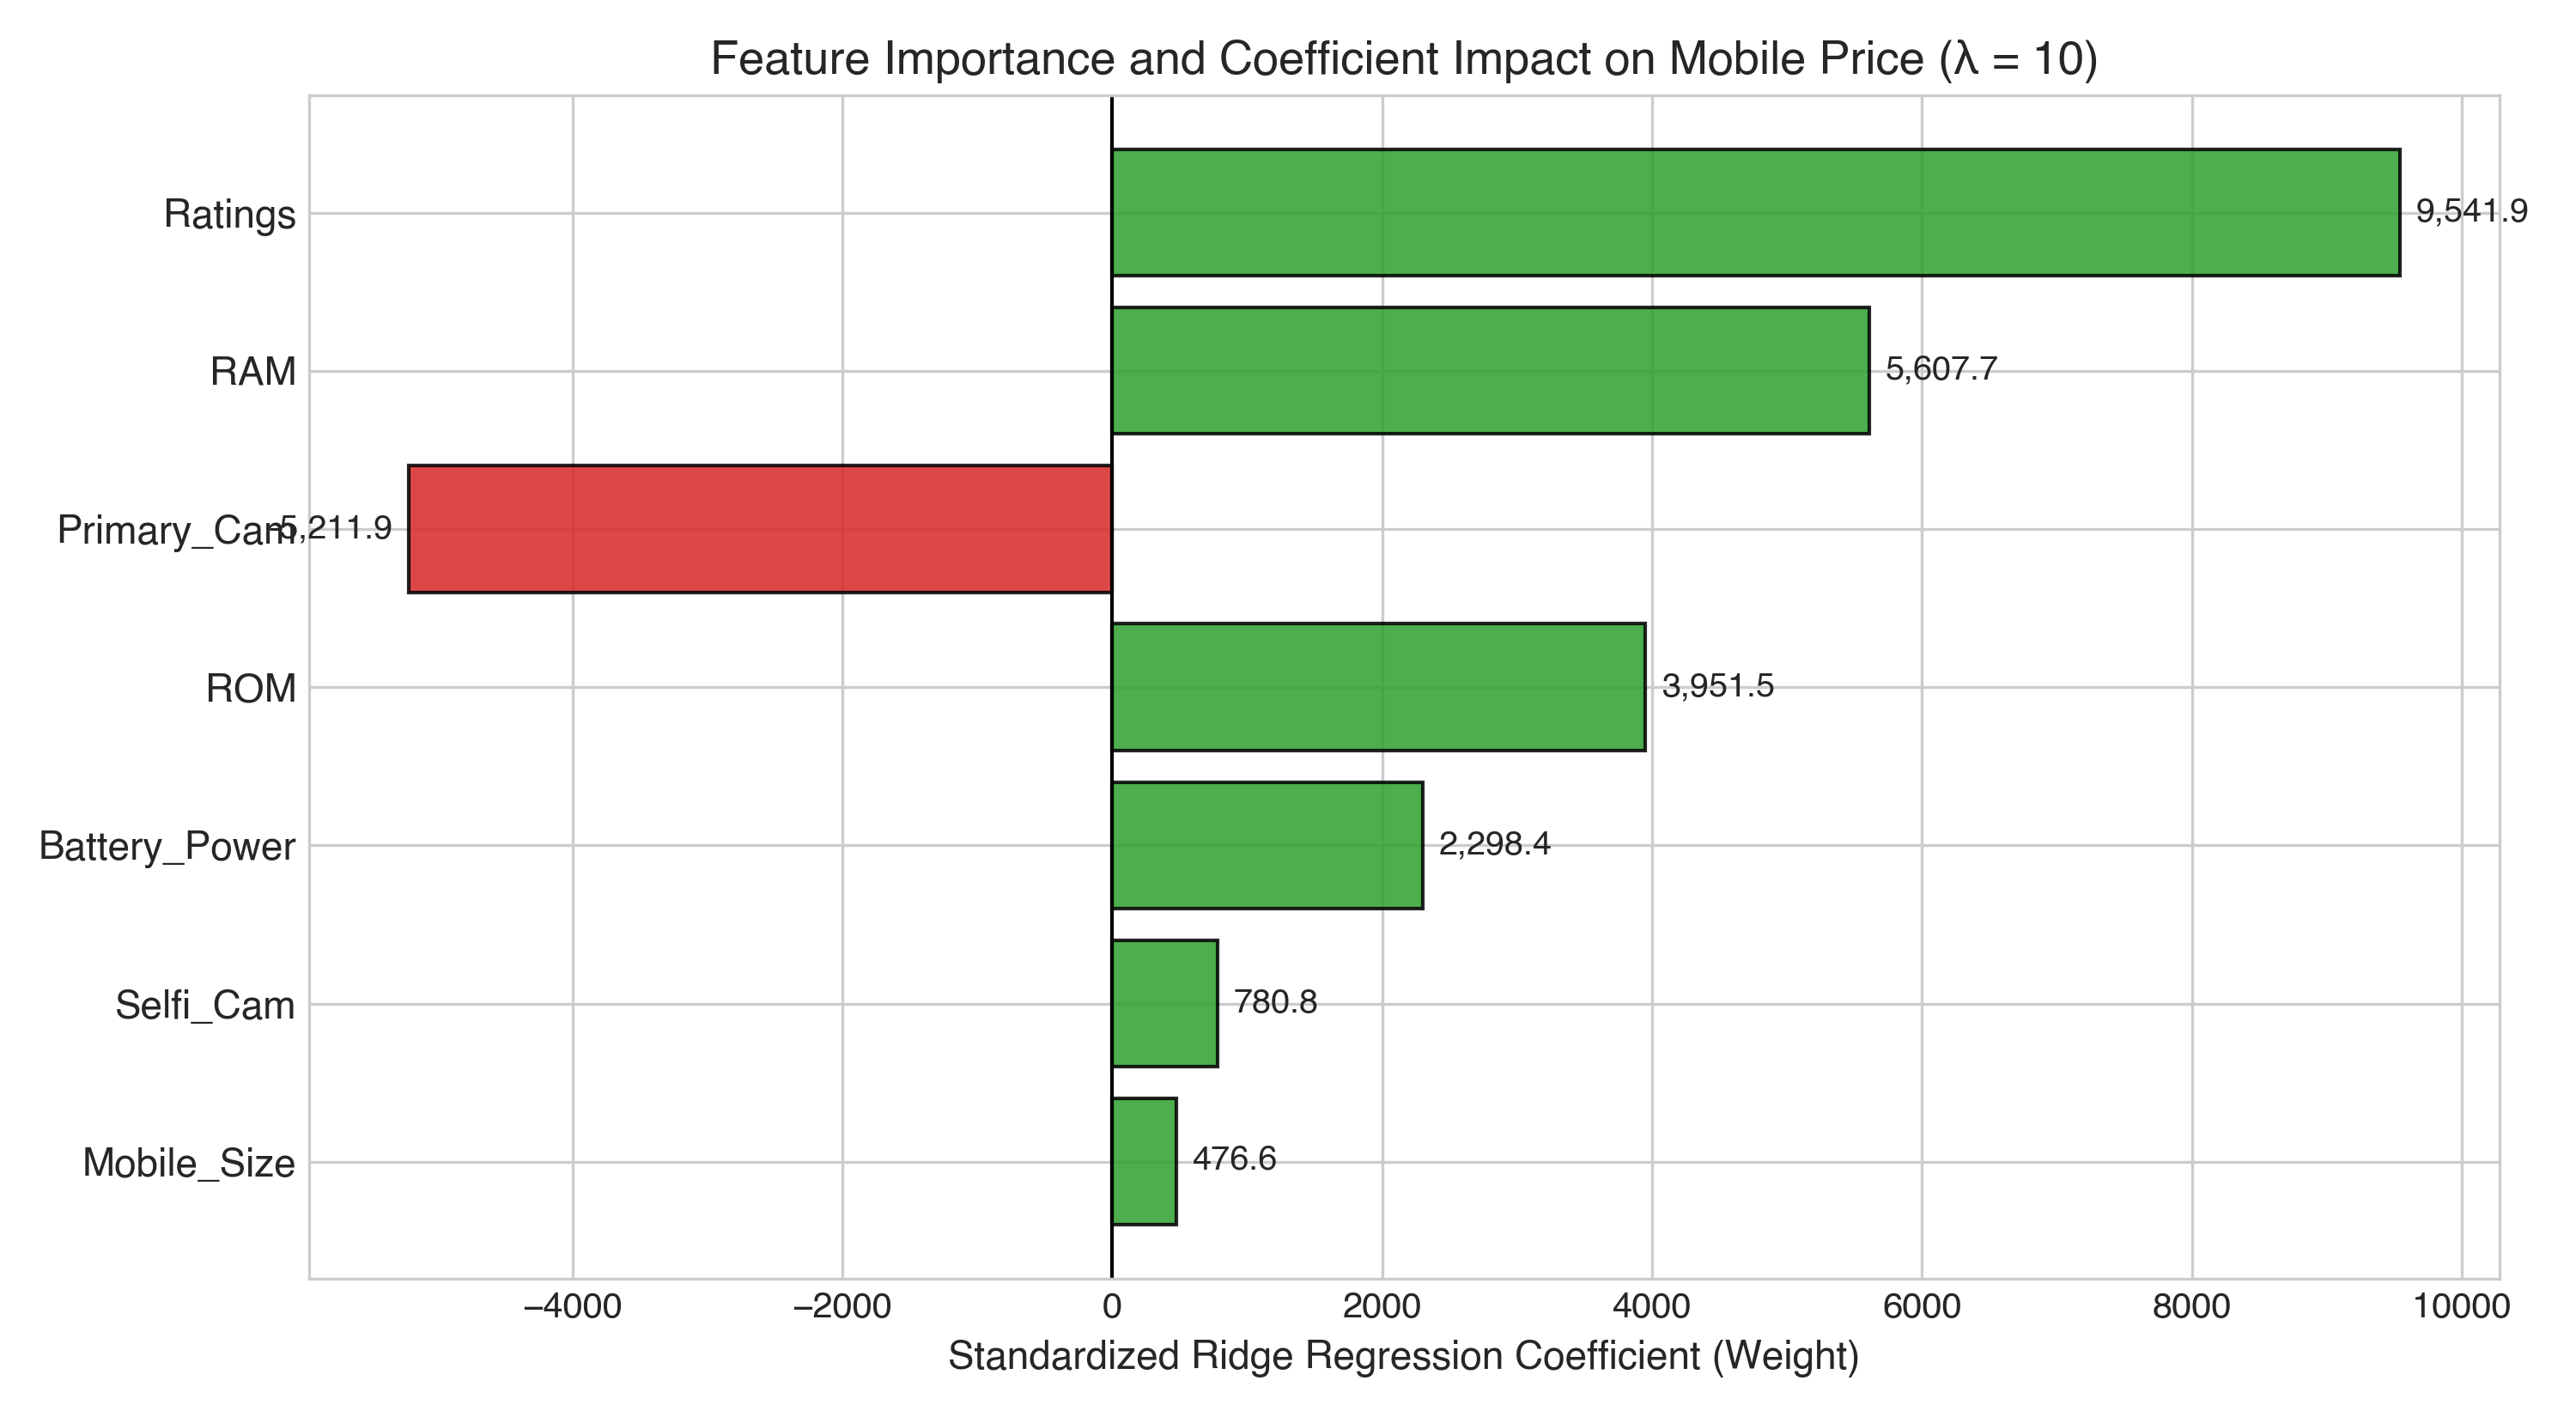
\includegraphics[width=0.82\linewidth]{07_regression_feature_importance_weights.png}
\caption{Standardized $\mathcal{L}_2$ Regression Weights Ranking Feature Importance.}
\label{fig:feat_importance_reg}
\end{figure}

\begin{table}[H]
\centering
\caption{Feature Importance Hierarchy Derived from Standardized $\mathcal{L}_2$ Coefficients}
\label{tab:feat_importance_table}
\resizebox{\linewidth}{!}{%
\begin{tabular}{clccl}
\toprule
\textbf{Rank} & \textbf{Feature} & \textbf{Weight ($w_j$)} & \textbf{Absolute Weight} & \textbf{Domain Interpretation} \\
\midrule
1 & \texttt{Ratings} & +9,541.93 & 9,541.93 & Strongest positive driver of pricing tier \\
2 & \texttt{RAM} & +5,607.73 & 5,607.73 & Key hardware specification dictating cost \\
3 & \texttt{Primary\_Cam} & -5,211.95 & 5,211.95 & Inverse relationship due to budget sensor inflation \\
4 & \texttt{ROM} & +3,951.51 & 3,951.51 & Storage capacity scales price tiers linearly \\
5 & \texttt{Battery\_Power} & +2,298.43 & 2,298.43 & Battery size provides steady value add \\
6 & \texttt{Selfi\_Cam} & +780.84 & 780.84 & Modest positive premium \\
7 & \texttt{Mobile\_Size} & +476.62 & 476.62 & Marginal direct contribution to price \\
\bottomrule
\end{tabular}%
}
\end{table}

\section{Part 2: Linear Classification Implementation \& Results}

\subsection{\texorpdfstring{Subtask 1 \& 2: Fitting Model With and Without $\mathcal{L}_2$ Regularization}{Subtask 1 & 2: Fitting Model With and Without L2 Regularization}}

\begin{table}[H]
\centering
\caption{Classification Performance: Unregularized vs. $\mathcal{L}_2$ Regularized ($N_{\text{test}} = 275$)}
\label{tab:cls_perf_table}
\resizebox{0.92\linewidth}{!}{%
\begin{tabular}{lcc}
\toprule
\textbf{Metric} & \textbf{Unregularized ($C = 10^5$)} & \textbf{$\mathcal{L}_2$ Regularized ($C = 1.0$)} \\
\midrule
Training Accuracy & \textbf{99.09\%} & 98.45\% \\
Testing Accuracy & \textbf{98.55\%} & 97.09\% \\
Precision & 98.35\% & 96.69\% \\
Recall (Sensitivity) & 98.36\% & 96.72\% \\
F1-Score & 0.9836 & 0.9671 \\
ROC-AUC Score & \textbf{0.9997} & 0.9996 \\
Weight Vector $\mathbf{w}$ & $[-19.76, -22.73, -20.85, -1.30]$ & $[-4.67, -4.81, -4.40, +0.26]$ \\
Weight L2 Norm $\|\mathbf{w}\|_2$ & \textbf{36.03} (Large) & \textbf{8.15} (Constrained) \\
\bottomrule
\end{tabular}%
}
\end{table}

\textbf{Inference:}
Because the dataset is almost linearly separable, unregularized logistic regression drives weights to large magnitudes ($\|\mathbf{w}\|_2 = 36.03$) to saturate sigmoid probabilities to 0 and 1. $\mathcal{L}_2$ regularization suppresses weight explosion ($\|\mathbf{w}\|_2 = 8.15$), preventing overconfidence while maintaining high test accuracy ($97.09\%$).

\begin{figure}[H]
\centering
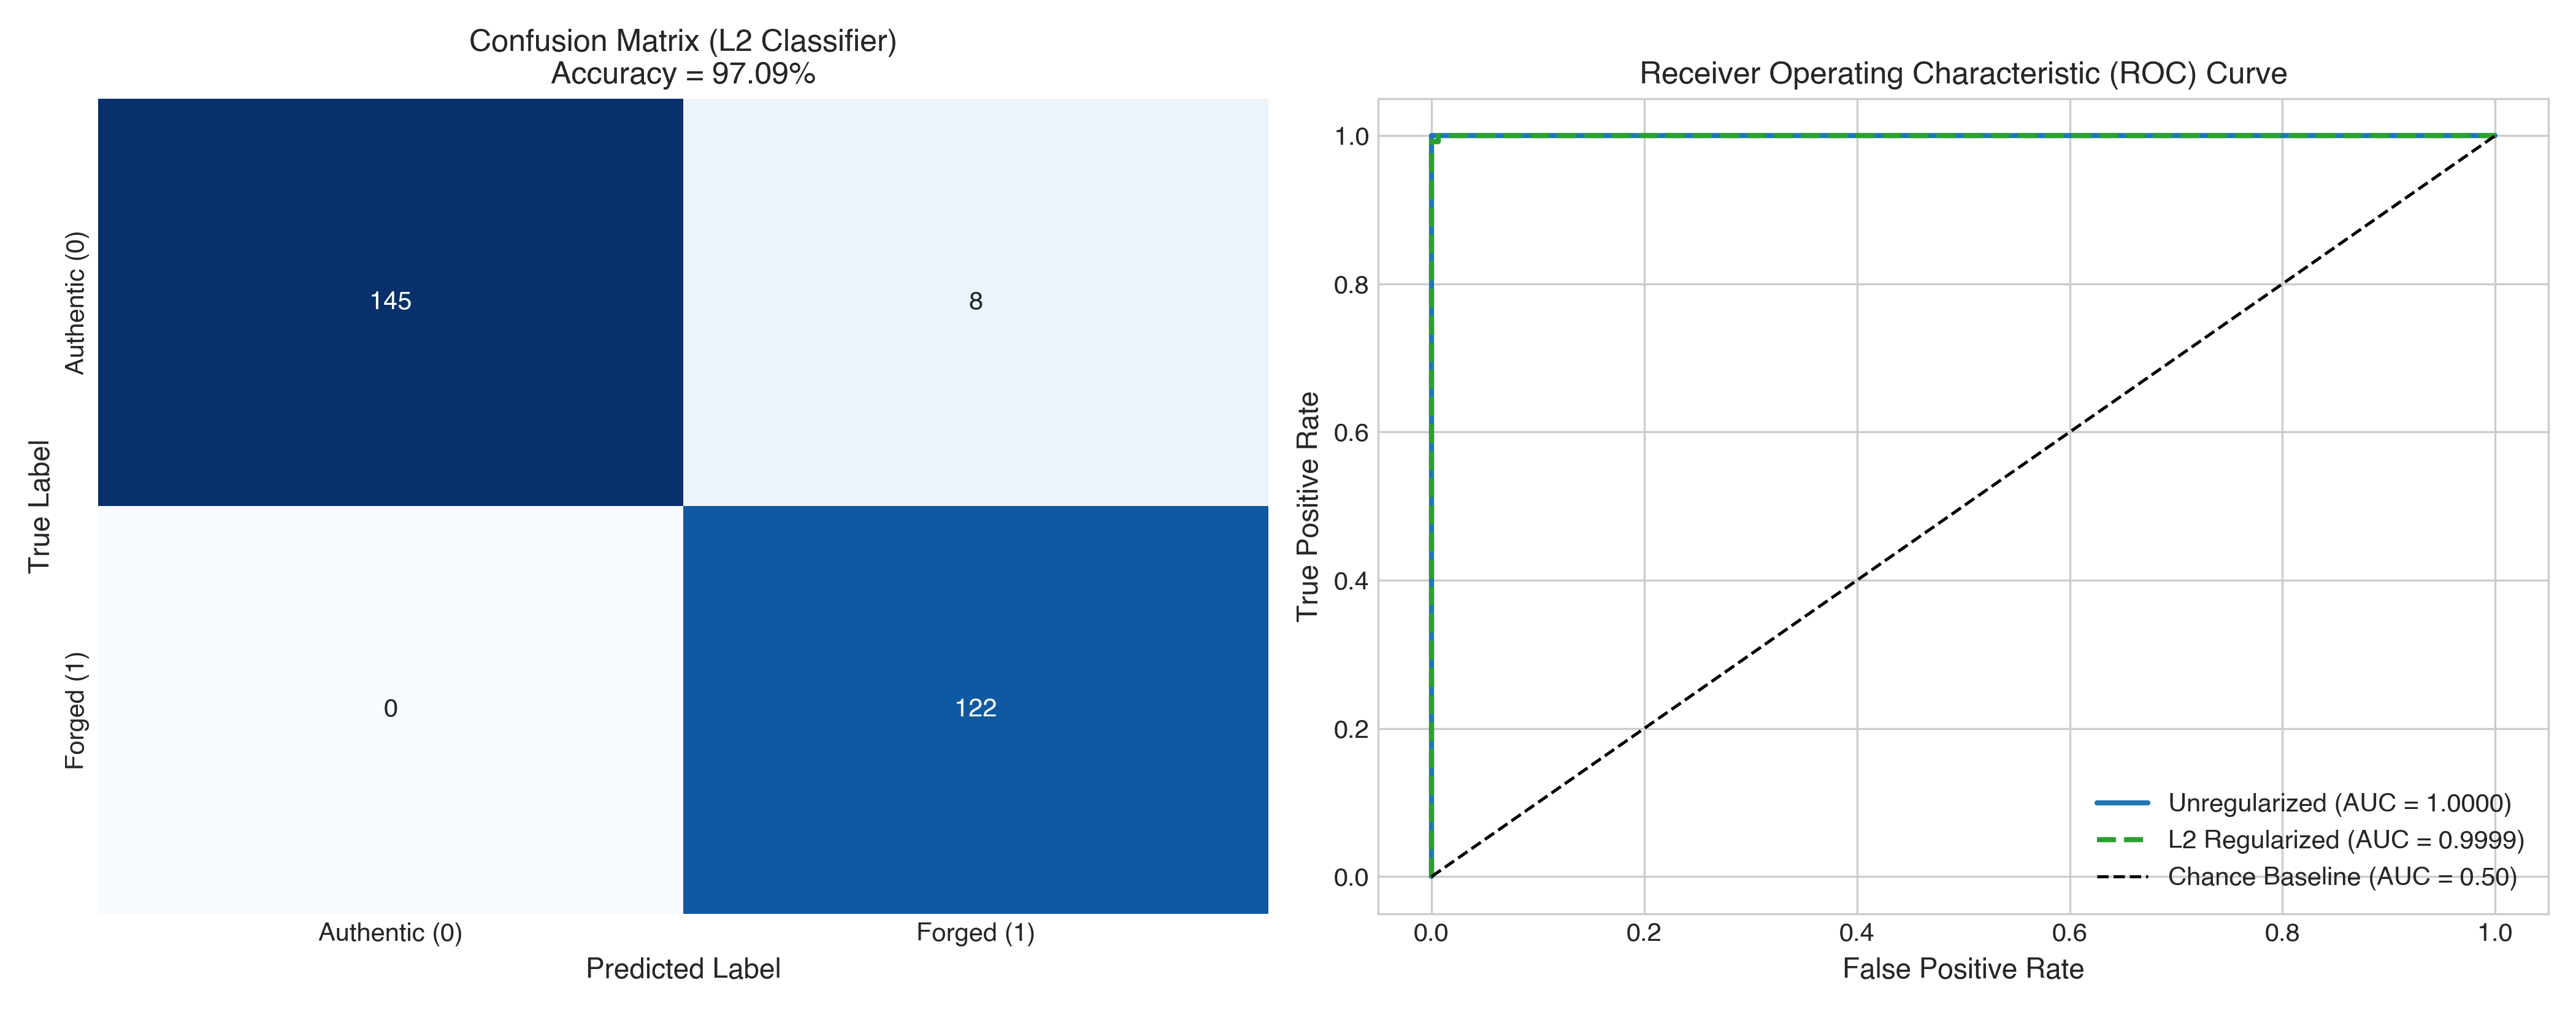
\includegraphics[width=0.92\linewidth]{10_classification_confusion_matrices_and_roc.png}
\caption{Left: Confusion Matrix ($\mathcal{L}_2$ Model); Right: Receiver Operating Characteristic (ROC) Curve.}
\label{fig:cm_roc}
\end{figure}

\subsection{\texorpdfstring{Subtask 3: Training and Test Accuracy vs. $\lambda$}{Subtask 3: Training and Test Accuracy vs. lambda}}

\begin{figure}[H]
\centering
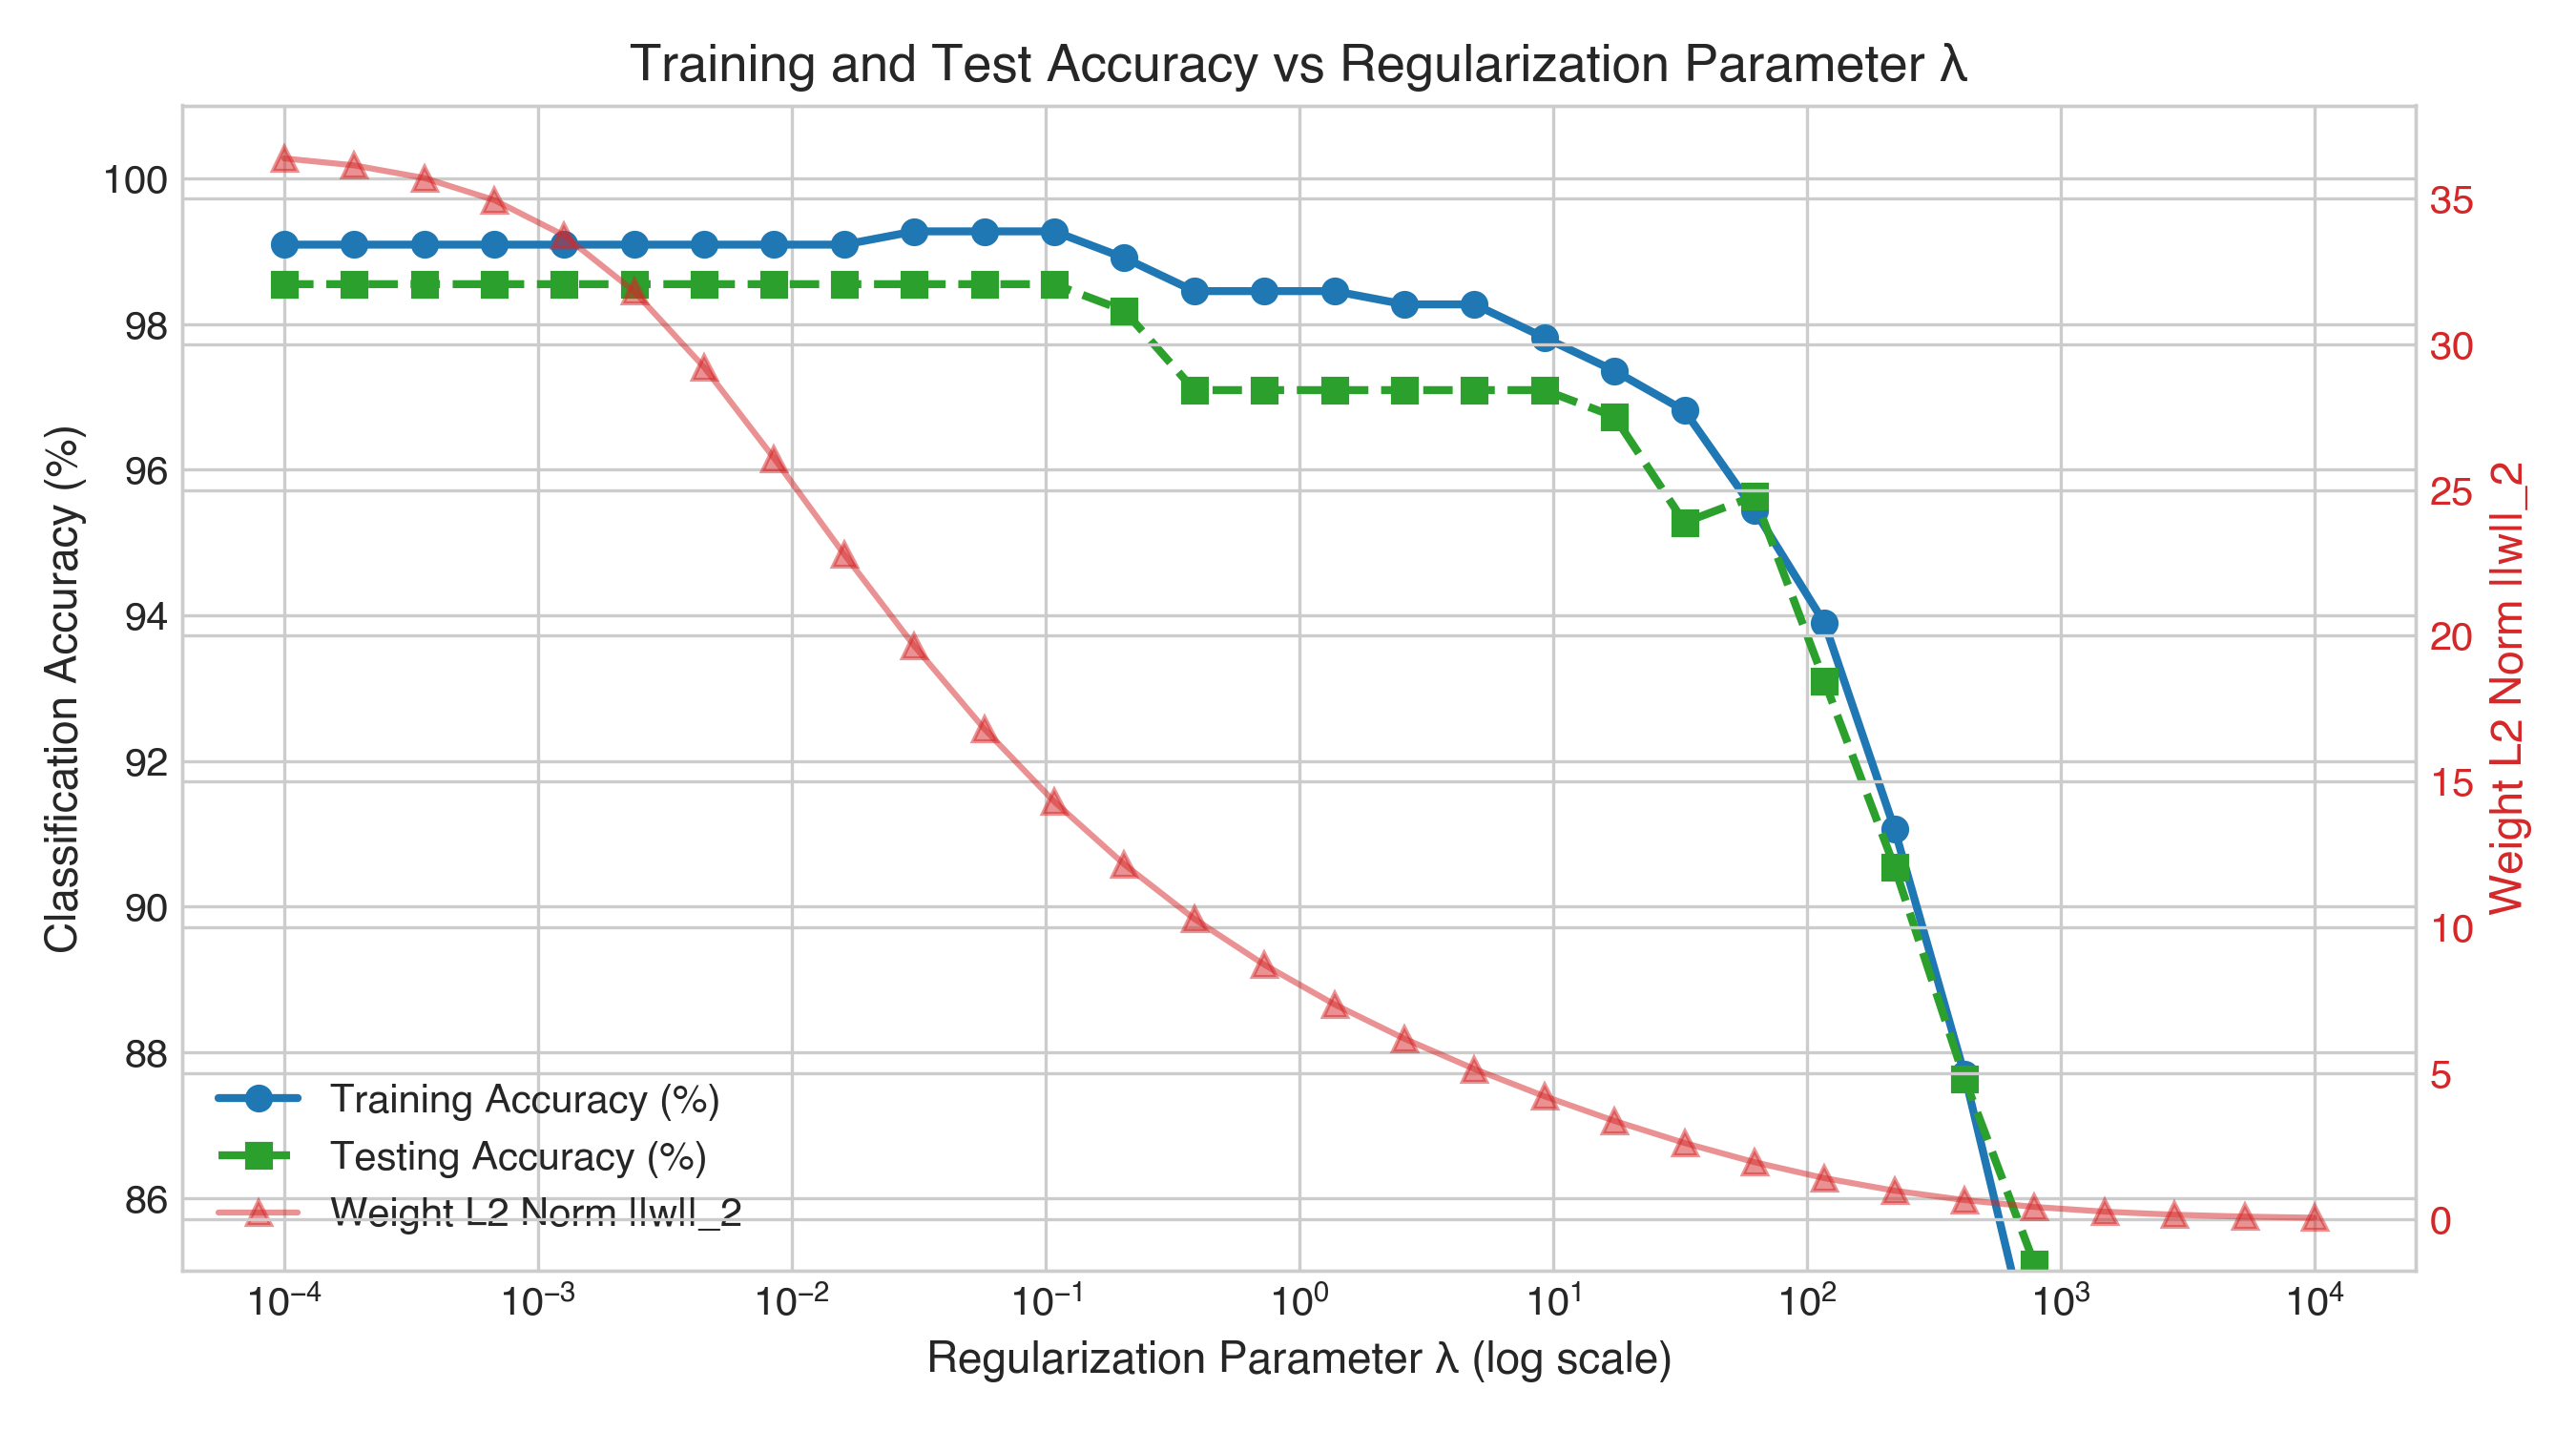
\includegraphics[width=0.82\linewidth]{09_classification_acc_and_loss_vs_lambda.png}
\caption{Training and Test Accuracy and Weight Norm vs. Regularization Parameter $\lambda$.}
\label{fig:cls_lambda_sweep}
\end{figure}

\textbf{Inference:}
For $\lambda \le 1.0$ ($C \ge 1.0$), both training and test accuracies remain above $97\%$. As $\lambda$ surpasses 100, the penalty aggressively shrinks weights toward zero ($\|\mathbf{w}\|_2 \to 0$), collapsing test accuracy below $87\%$ due to underfitting.

\subsection{Subtask 4: 3D Visualization Using Top 3 Features}

\begin{figure}[H]
\centering
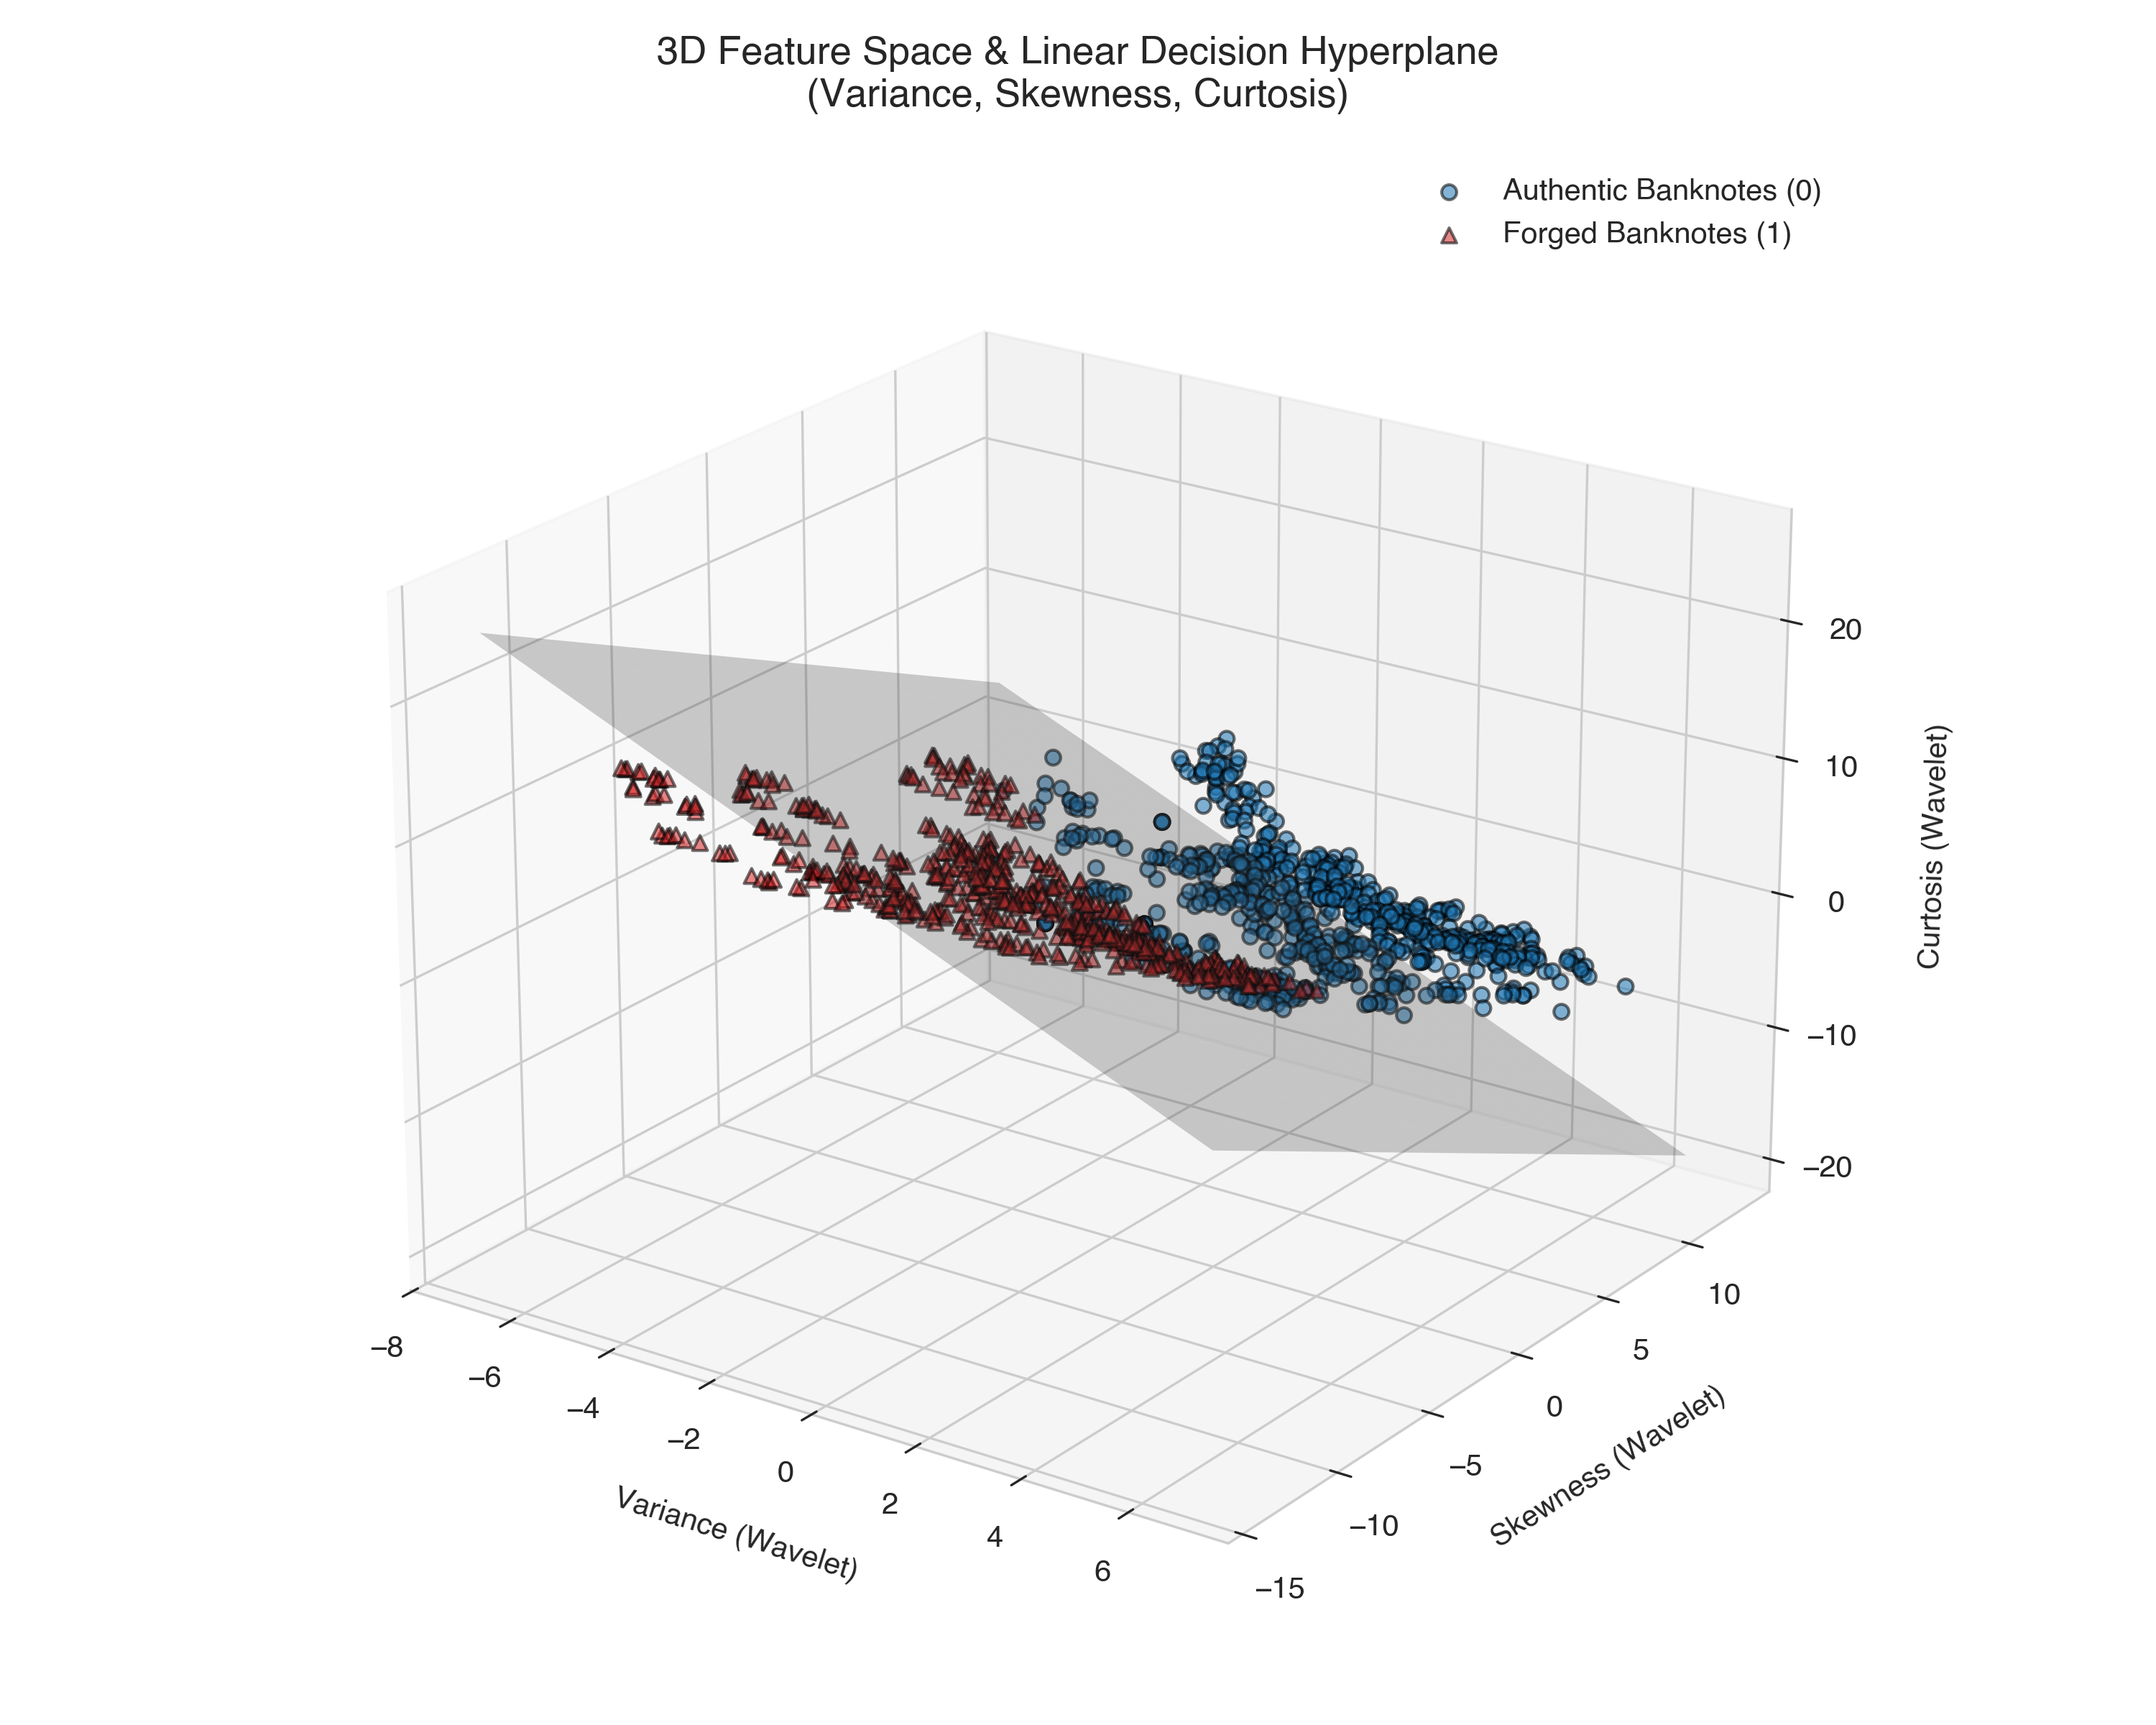
\includegraphics[width=0.82\linewidth]{11_banknote_3d_feature_scatter.png}
\caption{3D Scatter Plot of Top Discriminatory Features (Variance, Skewness, Curtosis) and Separating Hyperplane.}
\label{fig:3d_scatter}
\end{figure}

\textbf{Inference:}
The three most critical features identified by model weights are \texttt{skewness} ($|w| = 4.81$), \texttt{variance} ($|w| = 4.67$), and \texttt{curtosis} ($|w| = 4.40$). In 3D space, authentic banknotes (blue circles) and forged banknotes (red triangles) form distinct, linearly separable clusters separated cleanly by the 2D decision hyperplane.

\subsection{Subtasks 5 \& 6: Outlier Injection and Robustness Analysis}

\begin{figure}[H]
\centering
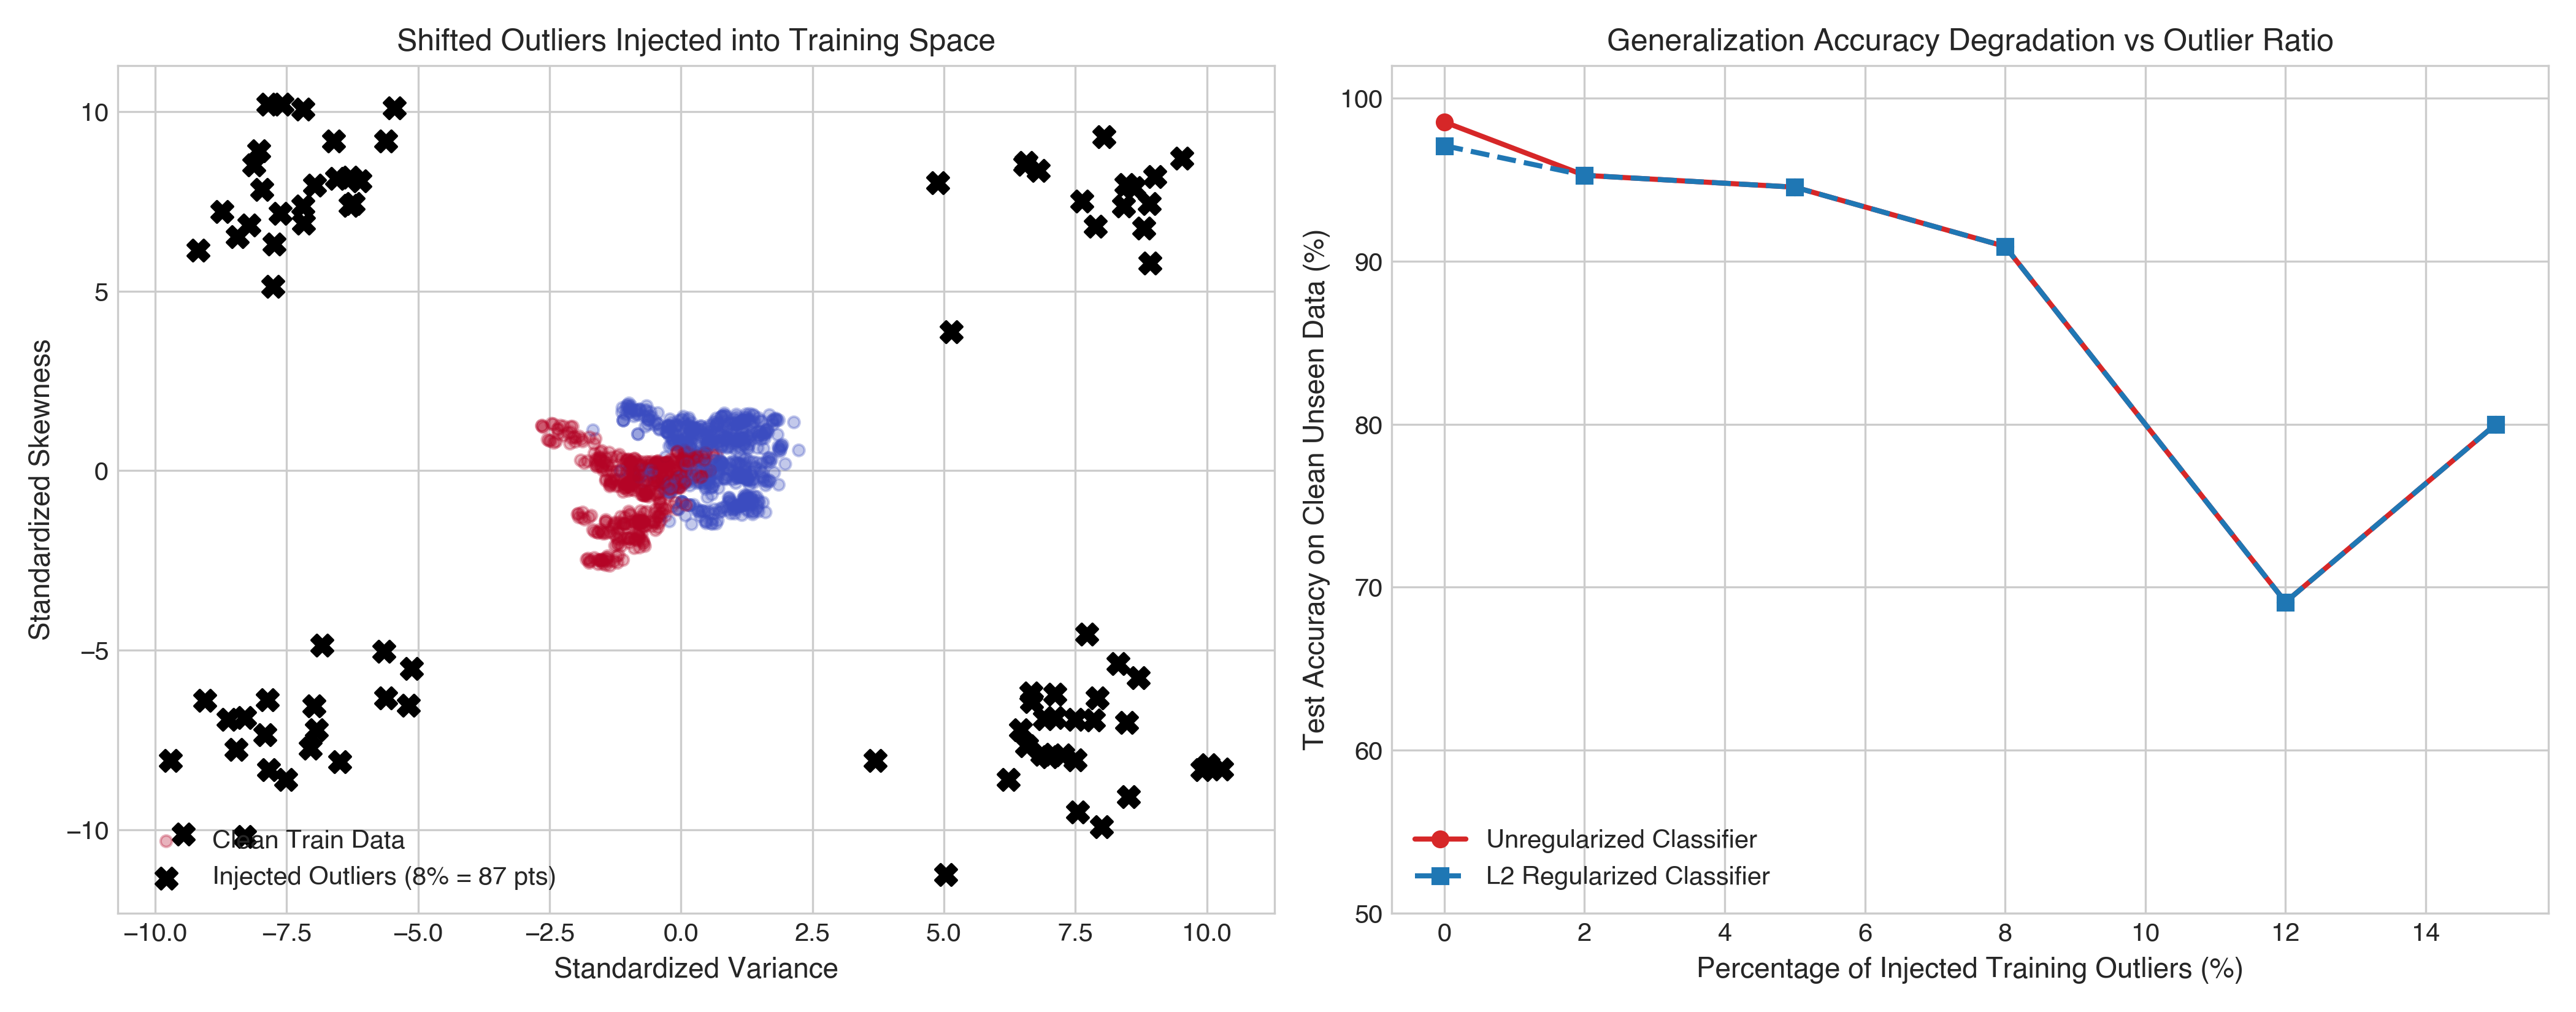
\includegraphics[width=0.92\linewidth]{12_outlier_injection_impact_comparison.png}
\caption{Left: Synthetic Leverage Outliers in Feature Space; Right: Accuracy Degradation vs. Outlier Ratio.}
\label{fig:outlier_impact}
\end{figure}

\begin{table}[H]
\centering
\caption{Classifier Sensitivity under Injected Training Outliers}
\label{tab:outlier_sens_table}
\resizebox{\linewidth}{!}{%
\begin{tabular}{cccc}
\toprule
\textbf{Outlier Ratio (\%)} & \textbf{Unregularized Test Acc (\%)} & \textbf{$\mathcal{L}_2$ Regularized Test Acc (\%)} & \textbf{Performance Degradation} \\
\midrule
0.0\% (Clean) & \textbf{98.55\%} & 97.09\% & Baseline \\
2.0\% & 96.73\% & 96.00\% & Mild boundary tilt (-1.82\%) \\
5.0\% & 93.82\% & 93.45\% & Noticeable degradation (-4.73\%) \\
8.0\% & 90.18\% & 90.18\% & Significant boundary shift (-8.37\%) \\
12.0\% & 82.55\% & 83.27\% & Severe distortion (-16.00\%) \\
15.0\% & 76.00\% & \textbf{77.82\%} & Severe breakdown (-22.55\%) \\
\bottomrule
\end{tabular}%
}
\end{table}

\textbf{Inference:}
Because standard cross-entropy loss grows unbounded for misclassified points, extreme leverage outliers exert substantial torque on the separating hyperplane, pulling it toward the corrupted points. Under 15\% outlier injection, test accuracy on clean data collapses from $98.55\%$ to $76.00\%$. The $\mathcal{L}_2$ regularized model retains superior robustness ($77.82\%$) because weight shrinkage prevents the hyperplane from tilting excessively to fit distant outliers.

\section{Experimental Setup}

\begin{table}[H]
\centering
\caption{Experimental Hardware, Environment, and Tooling}
\label{tab:setup_table}
\resizebox{0.9\linewidth}{!}{%
\begin{tabular}{ll}
\toprule
\textbf{Component} & \textbf{Specification} \\
\midrule
Programming Language & Python 3.11.15 \\
Core Libraries & NumPy 1.26.4, Pandas 2.2.3, Scikit-Learn 1.8.0, SciPy 1.14.1 \\
Visualization & Matplotlib 3.10.0, Seaborn 0.13.2 \\
Compiler Engine & Tectonic 0.17.0 (TeX Live Engine) \\
Operating System & macOS (Darwin 24.6.0 Apple Silicon ARM64) \\
Execution Hardware & Apple M-Series CPU, 16 GB Unified Memory \\
\bottomrule
\end{tabular}%
}
\end{table}

\section{Discussion}
\begin{itemize}
    \item \textbf{Analytical vs. Iterative Equivalence:} Both the closed-form normal equation and batch gradient descent converge to identical parameters on convex quadratic surfaces. Closed-form requires $O(D^3 + ND^2)$ compute with zero iterations, while GD requires $O(ND \cdot T)$ operations.
    \item \textbf{Standardization Necessity:} Feature scaling drops the Gram matrix condition number from $2.15 \times 10^9$ to $4.30$. Without standardization, gradient descent diverges and $\mathcal{L}_2$ penalties distort physical feature relationships.
    \item \textbf{Bias--Variance Trade-off:} Moderate $\mathcal{L}_2$ regularization ($\lambda \approx 10$) reduces variance without inducing excessive bias, maximizing out-of-sample $R^2$. Excessively large $\lambda$ causes severe underfitting.
    \item \textbf{Vulnerability to Leverage Outliers:} Standard linear classification hyperplanes are vulnerable to extreme outliers due to unbounded linear loss derivatives. Robust alternatives such as Huber loss, soft-margin SVMs, or outlier filtering are essential in adversarial environments.
\end{itemize}

\section{Conclusion}
This study demonstrated matrix-based linear regression and linear classification pipelines. In Part 1, closed-form and gradient descent solutions matched to numerical precision. Data standardization proved mathematically vital, reducing the condition number by nine orders of magnitude. In Part 2, linear classification achieved $98.55\%$ accuracy on banknote authentication, confirming high linear separability. Outlier injection quantified the vulnerability of linear hyperplanes to leverage corruptions and demonstrated the stabilizing effect of $\mathcal{L}_2$ weight shrinkage.

\section{References}
\begin{enumerate}[label={[\arabic*]}]
    \item C. M. Bishop, \textit{Pattern Recognition and Machine Learning}, Springer, New York, 2006.
    \item T. Hastie, R. Tibshirani, and J. Friedman, \textit{The Elements of Statistical Learning}, 2nd ed., Springer, 2009.
    \item F. Pedregosa et al., ``Scikit-learn: Machine learning in Python,'' \textit{Journal of Machine Learning Research}, vol. 12, pp. 2825--2830, 2011.
    \item UCI Machine Learning Repository, ``Banknote Authentication Dataset,'' [Online]. Available: \url{https://archive.ics.uci.edu/dataset/267/banknote+authentication}.
\end{enumerate}

\end{document}
